% Loaded before the class so that IEEEtran's internal font probes resolve in T1
% rather than the engine-default TU encoding (removes spurious substitutions
% under XeTeX/tectonic).
\RequirePackage[T1]{fontenc}
\documentclass[conference]{IEEEtran}

\usepackage[utf8]{inputenc}
\usepackage{cite}
\usepackage{amsmath}
% Times-compatible math so that symbols match IEEEtran's Times text face
% (newtxmath also supplies the AMS symbol set, so amssymb must NOT be loaded).
\usepackage[varvw]{newtxmath}
\usepackage{graphicx}
\usepackage{booktabs}
\usepackage{multirow}
\usepackage{makecell}
\usepackage{array}
\usepackage{tabularx}
\usepackage{siunitx}
\usepackage{url}
\usepackage{xcolor}
% Improves justification in IEEE's narrow columns (fewer under/overfull boxes).
\usepackage[protrusion=true,expansion=false]{microtype}

\sisetup{
  range-phrase = {\,--\,},
  range-units  = single,
  detect-weight = true,
  detect-family = true,
  separate-uncertainty = true,
}

% Uniform row height for the multi-line table headers used in Section V.
\renewcommand{\theadfont}{}
\renewcommand{\cellalign}{cc}

% ============================================================
\title{Anchored Conditionally-Gated Control for Wheeled Bipedal Balance and Disturbance Recovery}

\author{
\IEEEauthorblockN{Van Thuong Nguyen}
\IEEEauthorblockA{
Independent Researcher\\
Email: nvthuong180702@gmail.com
}
}

% Table notes: \centering (set by the table env) leaves \rightskip/\parfillskip
% at fil, which centres every last line. \tabnote restores normal justification.
% The 2em of \rightskip stretch is not cosmetic: notes carry unbreakable
% \path{} and \texttt{} filenames, and in a full-justified column those force
% badness-10000 underfull lines with visibly gaping interword space. A little
% permitted raggedness absorbs them instead.
\newcommand{\tabnote}{\par\leftskip=0pt\rightskip=0pt plus 2em%
  \parfillskip=0pt plus 1fil\relax}

\begin{document}

\maketitle

% ============================================================
\begin{abstract}
Wheeled bipedal robots face a fundamental trade-off: stiffness for sub-millimeter precision shrinks push-recovery capture, while integral action that cancels equilibrium bias winds up during disturbances.
We present the Anchored Conditionally-Gated Controller (ACC), a two-channel torque assembly whose core mechanism is a proximity-gated anchor: a position integral confined to a \SI{15}{cm} neighborhood, enabled by an asymmetric envelope follower ($\tau_{\text{attack}}{\approx}\SI{23}{ms}$, $\tau_{\text{release}}{\approx}\SI{1.5}{s}$) that distinguishes quiet stance from post-push ringdown.
ACC delivers omnidirectional push recovery ($F_{\min}{=}\SI{83}{N}$, $F_{\text{med}}{=}\SI{117}{N}$, \num{8}-direction sweep, $N{=}10$) together with sub-millimeter quiet-stance precision. We report accuracy (RMS from commanded home) and repeatability (RMS about the trial mean) separately, and resolve both on the sagittal axis---the actuated inverted-pendulum direction---rather than pooling them into a planar norm diluted by an axis this class of platform cannot drive. Under idealized conditions (clean sensors, \SI{0}{ms} delay, stiff contact, MuJoCo), ACC holds $0.294{\pm}0.015$\,mm sagittal repeatability ($N{=}10$), a $59{\times}$ improvement over a proportional-only baseline measured under one unified protocol. Accuracy is a full order of magnitude worse on the same axis: the robot parks $\SI{27.0}{mm}$ from the commanded home and then holds that offset to \SI{0.009}{mm}, and we report this gap as the design's principal open weakness rather than averaging it away. A factorial ablation ($N{=}10$ per row) separates the two: the gated damping terms produce the steadiness (removing the boost costs a factor of \num{16} in sagittal repeatability), while the anchor integral produces \SI{4.2}{mm} of the accuracy at a $3{\times}$ cost in steadiness; the proximity gate and asymmetric envelope are inert during quiet stance and decisive only under disturbance. Precision degrades by a factor of \num{5.5} at \SI{10}{ms} actuation delay, and to a hardware-projected \SIrange{1}{3}{mm} once encoder quantization, backlash, stiction, and IMU noise are accounted for; $F_{\max}$ bifurcates from \SI{96}{N} to \SI{47}{N} at any non-zero delay.
Six classical baselines---four 4-state TWIP variants (LQR, LQR+AW, LQR-DT, PI+AW) and two 6-state coupled variants (servo and direct-torque)---all fail (\SI{100}{\percent} fall rate, $N{=}20$--$60$); a preliminary PPO baseline (5.4M steps, single seed) suffers an \SI{85}{\percent} fall rate over multi-height transitions; removing the PID servo path (4-state Direct Torque LQR) improves survival by ${\sim}$\SI{38}{\percent} but does not prevent the fall.
Flight recovery (\SI{100}{cm} drop, \SI{50}{cm} ledge) and per-leg terrain adaptation (\SIrange{10}{20}{cm} one-wheel curb) are demonstrated at $N{=}10$ per condition and ablated: the per-leg height split is necessary at every curb height tested (\num{0}/\num{10} without it), whereas the airborne wheel-torque override proves to be a variance-bounding refinement rather than an enabling mechanism at these scales---a negative result we report explicitly. Core claims rest on $N{\geq}5$.
\end{abstract}
\begin{IEEEkeywords}
Wheeled biped robot, conditionally-gated control, anchored standing, proximity-gated integral, push recovery, flight recovery, terrain adaptation.
\end{IEEEkeywords}

% ============================================================
\section{Introduction}
\label{sec:intro}
% ============================================================

Wheeled biped robots need millimeter-level standing precision, omnidirectional push recovery, and terrain adaptation---but no single classical controller integrates all three: LQR handles balance~\cite{klemm2019ascento}, WBC posture~\cite{klemm2020lqrwbc}, MPC terrain~\cite{skater2024}, and RL locomotion~\cite{hwangbo2019rl}.

The difficulty is fundamental: lowering $k_p$ widens the capture basin at the cost of balance stiffness; omitting integral action leaves a \SI{1.3}{Nm} equilibrium bias that sustains a persistent, predominantly \emph{sagittal} limit cycle regardless of $k_p$ (measured at $N{=}10$: \SI{69.7}{mm} peak-to-peak sagittally against \SI{13.4}{mm} laterally, \SI{49.1}{mm} planar RMS from the commanded pose)---the oscillation lies on the one axis the wheels can drive, which is both why it persists and why it is the axis every mechanism in this paper is aimed at---yet a global integral winds up during pushes.

Preliminary PPO training (5.4M steps, single seed, in our \texttt{BalanceEnv}) showed limited height generalization: the policy stood at a single height (Surv ${\approx}\SI{3.20}{s}$, vs.\ \SI{0.52}{s} for LQR) but failed to generalize across \SIrange{0.40}{0.70}{m} base-$z$ (\S\ref{sec:height_convention})---height RMSE ${>}\SI{50}{mm}$, \SI{85}{\percent} falls on squat transitions---consistent with known difficulty of model-free RL on coupled pitch--height dynamics~\cite{xin2022centroidal}.

We present the Anchored Conditionally-Gated Controller (ACC), addressing both dilemmas through \emph{conditional activation}.
The core mechanism is a \textbf{proximity-gated anchor}: a position integral confined to a \SI{15}{cm} neighborhood, enabled by an \textbf{asymmetric envelope follower} ($\tau_{\text{attack}}{\approx}\SI{23}{ms}$, $\tau_{\text{release}}{\approx}\SI{1.5}{s}$) that distinguishes quiet stance from post-push ringdown.
Coupled with a \textbf{gated damping boost}, ACC achieves $0.294{\pm}0.015$\,mm repeatability on the sagittal axis---the actuated inverted-pendulum direction, and the one on which the limit cycle above lives---under idealized conditions (clean sensors, \SI{0}{ms} delay, $N{=}10$), at push performance equal to or better than the proportional-only baseline that carries no integral action at all. Absolute accuracy on that axis is a separate and weaker result, treated in Sec.~\ref{sec:standing}: the robot parks \SI{27.0}{mm} from the commanded home and then holds that offset to \SI{0.009}{mm}.

A factorial ablation measured under a single protocol (Table~\ref{tab:standing}) locates the mechanism more precisely than the gate structure suggests, and we state the result plainly because two of its three parts correct the intuitive attribution. First, the quiet-stance \emph{steadiness} comes from the gated \emph{damping} terms, not from the anchor integral: disabling the integral outright while leaving every gate intact leaves sagittal repeatability sub-millimeter (it in fact improves, \SI{0.294}{mm}$\rightarrow$\SI{0.089}{mm}), whereas reverting the two velocity-damping coefficients reinstates the full limit cycle (\SI{25.2}{mm}). What the integral buys is not steadiness but \emph{accuracy}---it removes \SI{4.2}{mm} of sagittal parking offset---and it buys that at a $3{\times}$ cost in steadiness. The two properties are produced by different mechanisms and trade against each other, which is why we report them as separate columns rather than as one planar number. Second, the proximity gate and the asymmetric envelope are provably inert during quiet stance---ablating either reproduces ACC bit-for-bit---because the robot never leaves the gate's inner band nor the envelope's release branch while standing still; their contribution is windup prevention and ringdown under disturbance, and only a displacement experiment can measure it. Third, the pitch safety gate is load-bearing even with no disturbance applied: removing it causes divergence from the initial-condition noise alone in \num{10}/\num{10} trials. The gates are thus enabling conditions that make an otherwise inadmissible damping and integral configuration safe, rather than the proximate source of the precision.
Six classical baselines---four 4-state TWIP variants (LQR, LQR+AW, LQR-DT, PI+AW) and two 6-state coupled variants (servo and direct-torque)---all fail (\SI{100}{\percent} fall rate), confirming that platform complexity, not servo lag alone, dominates the failure. Preliminary model-free PPO (5.4M steps, single seed) suffers an \SI{85}{\percent} fall rate; removing the PID servo path (Direct Torque LQR) yields only a ${\sim}$\SI{38}{\percent} improvement with persistent \SI{100}{\percent} falls.

The main contributions are:
\begin{enumerate}
    \item A \textbf{proximity-gated anchor} with asymmetric envelope follower achieving sub-millimeter idle precision without sacrificing omnidirectional push survival.
    \item A \textbf{two-channel conditionally-gated torque assembly} with flight recovery and per-leg terrain adaptation as independent extensions, each ablated at $N{=}10$---including the negative result that the flight override is not load-bearing at the reported drop scales.
    \item A \textbf{factorial ablation} (additive L0$\rightarrow$L3 $+$ subtractive S0$\rightarrow$S5) with six classical baselines (four 4-state-derived and two 6-state coupled) and a preliminary PPO baseline (5.4M steps, single seed).
\end{enumerate}


% ============================================================
\section{Related Work}
% ============================================================

\subsection{Wheeled Bipedal Platforms and Classical Control}
Ascento~\cite{klemm2019ascento} demonstrated two-wheeled jumping with LQR balancing, later extended to WBC with kinematic loops~\cite{klemm2020lqrwbc}.
Handle~\cite{boston_dynamics_handle2017} pioneered wheeled-leg coordination; Swiss-Mile~\cite{swissmile2021} combined driving with quadrupedal walking.
BITeno~\cite{wada2019biteno}, DIABLO~\cite{diablo2024}, Whleaper~\cite{whleaper2024} (closest to our morphology, uses LQR+PPO residual architecture), and SKATER~\cite{skater2024} applied LQR, PPO, and MPC for balancing and locomotion. Whleaper's LQR+PPO hybrid is the closest prior structured-controller-plus-learned-residual architecture; ACC targets the same paradigm with a stronger classical prior.
Zamani et al.~\cite{zamani2020coupled} demonstrated coupled pitch-roll LQR ($\theta_{\text{RMS}}{\approx}\SI{1.5}{\degree}$, $\phi_{\text{RMS}}{\approx}\SI{2.0}{\degree}$) on a rigid two-wheeled platform without articulated legs, where torque commands act directly on wheels---a structurally simpler control problem with fewer unstable modes and no leg-height dynamics. Our 6-state LQR replicates their coupled structure on a legged morphology and fails; the 4-state Direct Torque LQR---removing the servo path and re-optimizing roll gain ($k_{p,\text{roll}}{=}55.0$)---also fails (\SI{100}{\percent} fall rate, \SI{0.72}{s}). Both LQR variants use gains derived from a simplified 4-state TWIP model, not a full 10-DOF linearization of the articulated-leg plant (see Limitation~7); these results are therefore empirical---demonstrating that the specific LQR implementations tested fail---not a proof that LQR is structurally insufficient. Two facts---Zamani succeeds on a rigid two-wheeler, both our LQR variants fail on articulated legs---indicate that platform complexity (articulated legs, height dynamics), not servo lag alone, is the dominant factor differentiating Zamani's result.
Cascade control~\cite{cascade_standard,herzog2016wbc} and WBC~\cite{bellicoso2018wbc} use fixed-gain nested loops without conditional gates; gain scheduling~\cite{gain_scheduling_survey} varies parameters continuously with one variable rather than responding to qualitatively distinct physical regimes.
We additionally benchmarked a task-priority QP whole-body controller both standalone and as an assist layer on ACC (\S\ref{sec:wbc}); it fails to resolve the precision--recovery trade-off because its fixed task-priority formulation lacks conditional regime-gating.
Split-range, selector, and override architectures~\cite{shinskey1996,astrom2005advanced} already implement continuous blending in process control. ACC adopts this principle; its contribution is the synthesis of physically-motivated gating surfaces (spatial proximity, temporal velocity envelope, pitch safety-interlock) derived from wheeled-biped failure modes rather than generic process-variable limits.
ACC's conditional gates connect to hybrid/switched systems~\cite{liberzon2003switching}, where continuous dynamics are partitioned by discrete switching surfaces; smoothstep softens these to $C^1$ transitions.
A recent review~\cite{liu2024review} surveys wheel-legged biped platforms and control approaches, noting the absence of a unified classical solution.

\subsection{Disturbance Rejection, Anti-Windup, and ACC's Distinction}
DOB~\cite{ohnishi1993dob,chen2000dob,cui2019dob} and ADRC~\cite{han2009adrc,feng2023lqradrc} provide temporal disturbance estimation but cannot distinguish a push from post-push ringdown---both occupy the same frequency band.
Saturation-triggered conditional-integration AW triggers on actuator saturation; ACC's anchor uses \textbf{spatial, physics-conditioned gating}: the proximity gate confines integration to a \SI{15}{cm} neighborhood, and the asymmetric envelope distinguishes quiet stance from ringdown via velocity envelope---replacing the estimation-speed-vs-noise trade-off with a time-domain attack-vs-release trade-off.
Push recovery via capture-point~\cite{englsberger2015dcm,pratt2006capturepoint} and flight-phase control~\cite{roscia2023flight} is complementary.
Blind stair climbing via RL was shown on Ascento~\cite{chamorro2024stairclimbing}.
Terrain adaptation uses exteroceptive~\cite{legged_terrain_extero} or proprioceptive~\cite{blind_terrain_proprio,bellicoso2016terrain} sensing; ACC extends proprioceptive contact-point estimation to wheeled bipeds.
Gated control for humanoid balancing was explored by Hyon et al.~\cite{hyon2007gated}; ACC extends conditional gating to wheeled bipeds with continuous smoothstep transitions.

% ============================================================
\section{Robot Platform}
% ============================================================

\subsection{Robot Morphology and Simulation}
The robot (Fig.~\ref{fig:robot}) is a ten-DOF wheeled biped with five actuated joints per leg: hip roll (HR), hip yaw (HY), hip pitch (HP), knee (KN), and drive wheel (WH).
Mass: \SI{8.1}{kg}; thigh: \SI{0.26}{m}; shin: \SI{0.28}{m}; wheel radius: \SI{0.06}{m}; hip width: \SI{0.23}{m}.
Torque limits: \SI{30}{Nm} (HR, HY, WH), \SI{150}{Nm} (HP, KN).
MuJoCo~\cite{mujoco} simulation at \SI{500}{Hz} ($\Delta t_{\text{sim}}=\SI{0.002}{s}$). ACC controller: \SI{100}{Hz} ($\Delta t_{\text{ctrl}}=\SI{0.01}{s}$, \num{5} physics substeps); PPO and LQR baselines: \SI{50}{Hz} (\num{10} physics substeps), their own design rate, and additionally re-run rate-matched at \SI{100}{Hz} in \S\ref{sec:rate_matched}. All experiments use \SI{400}{Nm/s} torque rate limit, raw torque commands direct to actuators. MuJoCo integrator: implicitfast (4 iterations, 8 linesearch iterations); cone: pyramidal (elliptic for wheels, $\mu_s{=}1.2$, $\mu_k{=}0.8$ body); armature: \SI{0.008}{kg{\cdot}m^2} (wheels), \SI{0.02}{kg{\cdot}m^2} (leg joints); contact stiffness/damping: \texttt{solref}=\{0.002,1\} (body), \{0.005,0.7\} (wheels).
The stiff body contact (\texttt{solref}=\{0.002,1\}) idealizes a rigid ground. Softening \texttt{solref[0]} to 0.02 (tire-on-asphalt) increases planar idle RMS by ${\sim}$\SI{60}{\percent} to ${\sim}\SI{1.2}{mm}$, so every sub-millimeter idle figure reported here is conditional on stiff ground contact; tire compliance adds \SIrange{0.1}{0.5}{mm} on real surfaces (see \S\ref{sec:discussion}).

\subsubsection*{Height convention}
\label{sec:height_convention}
Two different vertical references appear in this paper and are easily confused,
so we fix them here and mark every height accordingly.
\textbf{CoM-$z$} is the height of the whole-body center of mass above ground and
is the quantity ACC commands and regulates; the nominal standing pose is
$h_{\text{CoM}}{=}\SI{0.404}{m}$.
\textbf{Base-$z$} is the torso root-body height, \texttt{qpos[2]} in the MuJoCo
model; the same nominal pose has $z_{\text{base}}{=}\SI{0.536}{m}$, i.e.\
\SI{13.2}{cm} above the CoM.
The offset is pose-dependent but varies by less than \SI{1}{cm} over the
postures used here, so the two conventions differ by roughly a constant.
All ACC results are reported in CoM-$z$.
The PPO baseline (\S\ref{sec:baselines}) commands base-$z$ over
\SIrange{0.40}{0.70}{m}, and the WBC baselines (\S\ref{sec:wbc}) inherit the
same base-$z$ convention; those numbers are labelled base-$z$ where they appear
and must not be compared numerically against CoM-$z$ heights.
Confusing the two is not hypothetical: it is exactly bug~F3 in our own WBC
implementation audit (Table~\ref{tab:wbc_bugs}), where base-$z$ was passed as a
CoM-$z$ command and produced a \SI{13.2}{cm} reference error.

ACC's posture map is calibrated at two setups, at CoM heights of \SI{0.354}{m}
and \SI{0.454}{m} ($\pm\SI{5}{cm}$ about nominal), and interpolated between
them. Outside that band the joint targets are linearly extrapolated, bounded to
the interval $[0.254, 0.554]\,$m, i.e.\ \SI{10}{cm} beyond the calibrated band at
each end. This $\pm\SI{10}{cm}$ extrapolation bound, and not a $\pm\SI{5}{cm}$
one, is what the per-leg height split (\S\ref{sec:terrain}) operates against.

\begin{figure}[t]
    \centering
    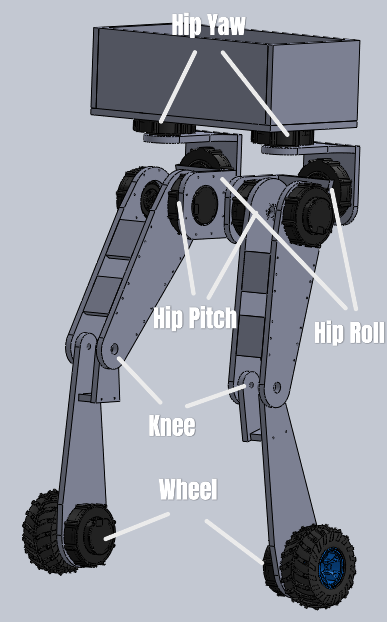
\includegraphics[width=\linewidth]{figures/annotated_robot_joints.png}
    \caption{Robot joint layout with world coordinate frame (right-handed, Z up). In the model as built, both wheel axles lie along world $X$ and the two wheel links are separated by \SI{0.271}{m} along $X$; the rolling---and therefore sagittal---direction is world $Y$, and world $X$ is the lateral (track) axis. All axis-resolved results in this paper follow that convention, verified four independent ways in Sec.~\ref{sec:standing}. The CoM is located at the torso geometric center. Each leg: hip roll (HR), hip yaw (HY), hip pitch (HP), knee (KN), wheel (WH).}
    \label{fig:robot}
\end{figure}

% ============================================================
\section{ACC Formulation}
% ============================================================

\subsection{Two-Channel Torque Assembly}
\label{sec:overview}

ACC assembles a PD balance core, proximity-gated anchor integral, and posture regulation into two torque channels---wheel torque ($\boldsymbol{\tau}_w\in\mathbb{R}^2$) and leg-joint torque ($\boldsymbol{\tau}_q\in\mathbb{R}^8$)---with flight and terrain as independent extensions (Fig.~\ref{fig:acc_arch}):

\begin{equation}
\begin{aligned}
\boldsymbol{\tau}_w &= \boldsymbol{\tau}_{\text{balance}} + g_{\text{anchor}}\boldsymbol{\tau}_{\text{anchor}} + g_{\text{flight}}\boldsymbol{\tau}_{\text{flight}},\\
\boldsymbol{\tau}_q &= \boldsymbol{\tau}_{\text{posture}}(h^{\text{cmd}}) + g_{\text{terrain}}\Delta\boldsymbol{\tau}_{\text{posture}}(h^{\text{cmd},L},\,h^{\text{cmd},R}).
\end{aligned}
\label{eq:two_channel}
\end{equation}

Every gate $g_*$ except the flight gate is a \emph{smoothstep} function of a physical condition (proximity, quietness, attitude, terrain disparity) rather than a discrete switch:

\begin{equation}
\operatorname{ss}(x;a,b) = 3t^2 - 2t^3,
\qquad t = \operatorname{clip}\!\left(\frac{x-a}{b-a},\,0,\,1\right).
\label{eq:smoothstep}
\end{equation}

Equation~\eqref{eq:smoothstep} is the standard Hermite blend: it is $C^1$ in $x$, with $\operatorname{ss}=0$ for $x\leq a$, $\operatorname{ss}=1$ for $x\geq b$, and zero derivative at both knees.
Continuity matters here for a concrete reason. A hard threshold on any of these conditions injects a torque step whose magnitude equals the full gated component; at \SI{100}{Hz} with a \SI{400}{Nm/s} rate limit, such a step is spread over several control cycles by the rate limiter and appears to the plant as an unmodelled impulse.
Smoothstep removes the step entirely: the gated component enters and leaves the torque sum with continuous first derivative, so the rate limiter is never the active constraint during a gate transition.
The one exception is $g_{\text{flight}}$, which is a genuinely discrete load-based hysteresis with asymmetric engage/release timers (\num{2}-step engage, \num{5}-step release); contact loss is a binary physical event, and the asymmetric timers exist specifically to prevent balance torque from re-engaging during landing bounce.
Note that the composition $g_{\text{env}} = 1 - \operatorname{ss}(\mathrm{EMA}(|v_{\text{sag}}|);\cdot)$ is only $C^0$ \emph{in time}, because the asymmetric EMA of Eq.~\eqref{eq:asym_ema} switches coefficients when $|v_t|$ crosses $\mathrm{EMA}_{t-1}$; the smoothstep is still $C^1$ in its argument, so the resulting torque is continuous but its time derivative may jump at attack/release transitions.

Wheel torques control sagittal balance and yaw; leg-joint torques control posture and per-leg height adaptation.
The two channels are coupled only through the plant, not through the controller: no term in $\boldsymbol{\tau}_w$ reads a leg-posture state and no term in $\boldsymbol{\tau}_q$ reads the sagittal balance state.
This is what allows flight recovery and terrain adaptation to be added as independent extensions (\S\ref{sec:flight}, \S\ref{sec:terrain}) without retuning the anchor.

\textbf{Relation to existing gated architectures.}
``Conditionally-gated'' here denotes smoothstep activation by \emph{physical} conditions ($g_{\text{prox}}$, $g_{\text{env}}$, $g_\theta$, $g_{\text{terrain}}$), and we make no claim that continuous blending is itself novel---split-range, selector, and override controllers have used it in process control for decades~\cite{shinskey1996,astrom2005advanced}.
Three distinctions are worth stating precisely.
First, industrial override architectures select \emph{among parallel controllers} using process-variable limits; ACC gates \emph{components within a single torque assembly} using physical regime.
Second, the gating variables are not control errors but physical quantities of three different kinds---spatial (distance from home), temporal (velocity envelope), and safety-interlock (attitude)---each chosen because a specific measured failure mode of this platform is expressible in it (\S\ref{sec:discussion}).
Third, ACC is not cascade control~\cite{cascade_standard}: there is no inner/outer loop hierarchy and no setpoint is passed between controllers.
The contribution is therefore the \emph{synthesis}---which gating surfaces, on which variables, with which asymmetry---not the blending mechanism.

\begin{figure}[t]
    \centering
    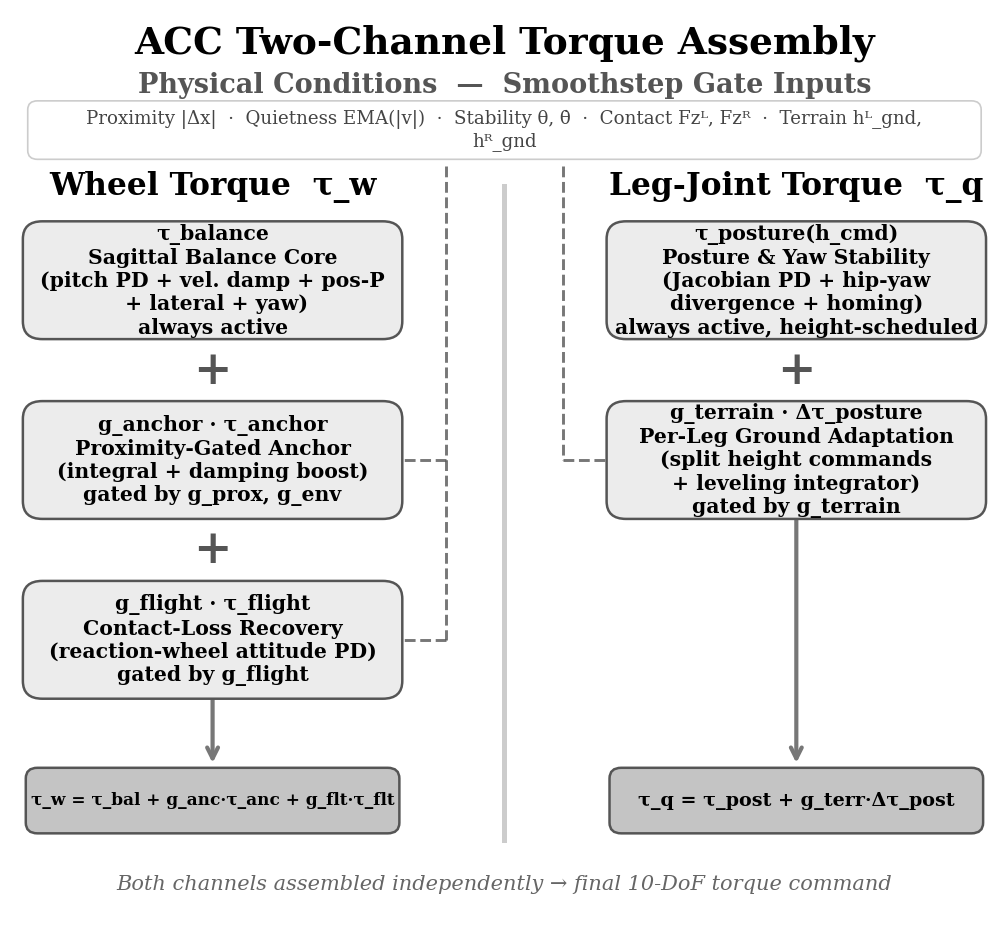
\includegraphics[width=\linewidth]{figures/acc_architecture.png}
    \caption{ACC two-channel torque assembly. Physical conditions gate each component via continuous smoothstep functions (dashed).}
    \label{fig:acc_arch}
\end{figure}

\subsection{Sagittal Balance Core ($\boldsymbol{\tau}_{\text{balance}}$)}
\label{sec:balance_core}

The sagittal balance component is always active and acts entirely in the wheel-torque channel:

\begin{equation}
\boldsymbol{\tau}_{\text{balance}} =
\begin{bmatrix}
\tau_{\text{com}} + \tau_{\text{diff}} \\
\tau_{\text{com}} - \tau_{\text{diff}}
\end{bmatrix},
\quad
\begin{aligned}
\tau_{\text{com}} &= \tau_{\text{pitch}} + \tau_{\text{damping}} + \tau_{\text{pos}},\\
\tau_{\text{diff}} &= \tau_{\text{lat}} + \tau_{\text{yaw}}.
\end{aligned}
\label{eq:balance}
\end{equation}

where $\tau_{\text{com}}$ and $\tau_{\text{diff}}$ are common-mode and differential components, respectively. The individual terms are:

\begin{align}
\tau_{\text{pitch}} &= k_p\cdot\theta + k_d\cdot\dot{\theta},\\
\tau_{\text{damping}} &= -k_{\text{vel}}\cdot v_{\text{sag}},\\
\tau_{\text{pos}} &= -k_{\text{pos}}\cdot\operatorname{clip}(\Delta x,\,\pm\SI{0.10}{m}),\\
\tau_{\text{lat}} &= k_{p,\text{roll}}\cdot\phi + k_{d,\text{roll}}\cdot\dot{\phi},\\
\tau_{\text{yaw}} &= k_{p,\text{yaw}}\cdot e_\psi + k_{d,\text{yaw}}\cdot\omega_z,
\end{align}

where $\theta$ is the torso pitch angle, $\dot{\theta}$ is the pitch rate, $v_{\text{sag}}$ is the sagittal body velocity, $\Delta x$ is the sagittal position error from the latched home position, $\phi$ is the roll angle, and $e_\psi$ is the yaw error.

\textbf{P-only limitation.}
The P position term ($k_{\text{pos}}$, clipped to $\pm\SI{0.10}{m}$, saturating at $\pm\SI{4}{Nm}$) keeps the robot within $\pm$\SIrange{4}{6}{cm} of home but leaves a \SI{1.3}{Nm} equilibrium bias sustaining a perpetual limit cycle---motivating the anchor integral.

\textbf{Why saturation-triggered anti-windup is insufficient.}
Saturation-triggered AW triggers on actuator saturation; on this platform the critical failure is \textbf{state-dependent}: during a push, position error grows to \SIrange{10}{30}{cm} while wheels remain within their \SI{20}{rad/s} range, so saturation-triggered AW never activates.
ACC's proximity gate provides spatial confinement via continuous smoothstep---avoiding both over-restriction (blocking slow-drift correction) and under-restriction (allowing windup during sustained pushes).
The simplest conditional-integration AW is evaluated in Appendix~\ref{sec:aw_supp}; broader AW families remain open.

\textbf{Pitch stiffness.}
Pitch stiffness is fixed at $k_p{=}50$ in the canonical ACC architecture. The anchor and boost alone resolve the precision-push trade-off without gain scheduling; a scheduled variant that softened $k_p$ from 50 to 35 during pushes was tested and rejected---it did not improve push survival (S0 vs.\ S1, Table~\ref{tab:push_ablation}) and is excluded from the canonical specification.

\subsection{Proximity-Gated Anchor Mechanism ($g_{\text{anchor}}\!\cdot\!\boldsymbol{\tau}_{\text{anchor}}$)}
\label{sec:anchor}

The anchor mechanism is the core contribution. It adds two terms to the wheel-torque channel that are active only when the robot is near home \emph{and} genuinely at rest:

\begin{equation}
\boldsymbol{\tau}_{\text{anchor}} =
K_i\!\int\! g_{\text{prox}}\cdot g_{\text{env}}\cdot(-\Delta x)\,dt \;+\;
g_{\text{boost}}\cdot K_{\text{boost}}\cdot(-v_{\text{sag}}),
\label{eq:anchor}
\end{equation}

where all gates are continuous smoothstep functions designed to equal $1$ when the robot is ``at home and quiet'' and transition smoothly to $0$ otherwise:

\begin{align}
g_{\text{prox}}(\Delta x) &= 1 - \operatorname{ss}\bigl(|\Delta x|;\;\SI{0.05}{m},\,\SI{0.15}{m}\bigr),
\label{eq:g_prox}\\[2pt]
g_{\text{env}}(v_{\text{sag}}) &= 1 - \operatorname{ss}\bigl(\mathrm{EMA}(|v_{\text{sag}}|);\;\SI{0.25}{m/s},\,\SI{0.50}{m/s}\bigr),
\label{eq:g_env}\\[2pt]
g_\theta(\theta,\dot{\theta}) &= \bigl[1 - \operatorname{ss}(|\theta|;\,\SI{2}{\degree},\,\SI{12}{\degree})\bigr] \nonumber\\
&\quad\times \bigl[1 - \operatorname{ss}(|\dot{\theta}|;\,\SI{2}{\degree/s},\,\SI{15}{\degree/s})\bigr],
\label{eq:g_theta}\\[2pt]
g_{\text{boost}} &= g_{\text{prox}}\cdot g_{\text{env}}\cdot g_\theta,
\label{eq:g_boost}
\end{align}

where $\operatorname{ss}(x;a,b)$ denotes the smoothstep of Eq.~\eqref{eq:smoothstep} with lower and upper knees $a$ and $b$.
Each gate is therefore a dimensionless, monotone, $C^1$ function that equals $1$ inside its ``home and quiet'' band, falls smoothly to $0$ outside it, and never switches discontinuously.
Three physically distinct conditions must hold simultaneously for the anchor to integrate: the robot must be spatially near home ($g_{\text{prox}}$), temporally quiet ($g_{\text{env}}$), and attitudinally settled ($g_\theta$).

The pitch stability gate $g_\theta$ closes when either pitch or pitch rate exceeds its band, preventing the damping boost from fighting a gentle sustained push that does not trigger the velocity envelope.
When the robot is genuinely at rest ($|\theta|<\SI{2}{\degree}$, $|\dot{\theta}|<\SI{2}{\degree/s}$), $g_\theta=1$ and the boost is fully available.

\textbf{Asymmetric envelope follower.}
The key to reliable quiet-stance detection is the asymmetric exponentially-weighted moving average (EMA) of $|v_{\text{sag}}|$:
\begin{equation}
\text{EMA}_t = \begin{cases}
\alpha_a|v_t| + (1{-}\alpha_a)\text{EMA}_{t-1}, & \text{if } |v_t| > \text{EMA}_{t-1},\\
\alpha_r|v_t| + (1{-}\alpha_r)\text{EMA}_{t-1}, & \text{otherwise},
\end{cases}
\label{eq:asym_ema}
\end{equation}
with time constants $\tau_{\text{attack}}{\approx}\SI{23}{ms}$ and $\tau_{\text{release}}{\approx}\SI{1.5}{s}$ as the primary specification; the discrete coefficients are derived via $\alpha_a=1-\exp(-\Delta t / \tau_{\text{attack}})\approx 0.35$ and $\alpha_r=1-\exp(-\Delta t / \tau_{\text{release}})\approx 0.007$ at \SI{100}{Hz} ($\Delta t{=}\SI{0.01}{s}$).
This asymmetry is essential: a symmetric EMA is \emph{bistable}---post-push oscillation holds the EMA in a middle band where the gate is half-open and the boost cannot collapse the cycle (validated by the symmetric-EMA ablation, Section~\ref{sec:results}).
The fast-attack/slow-release envelope jumps to $1$ only when oscillation truly decays, and drops to $0$ within $\sim\SI{25}{ms}$ of a disturbance. The concept traces to peak-hold and envelope-detector circuits~\cite{astrom2005advanced}; ACC's innovation is coupling envelope detection to a spatial proximity gate for integral conditioning. Fig.~\ref{fig:gate_activation} illustrates the complete gate activation sequence during a push-recovery cycle.

\textbf{EMA initialization.}
EMA$_0{=}0$ biases $g_{\text{env}}{\approx}1$ for $\sim$\SI{7.5}{s} at startup, decaying as velocity noise accumulates.
Measurements use \SIrange{3}{5}{s} settle (see Table captions); hardware should initialize $\text{EMA}_0{=}1.0$.

\begin{figure*}[t]
    \centering
    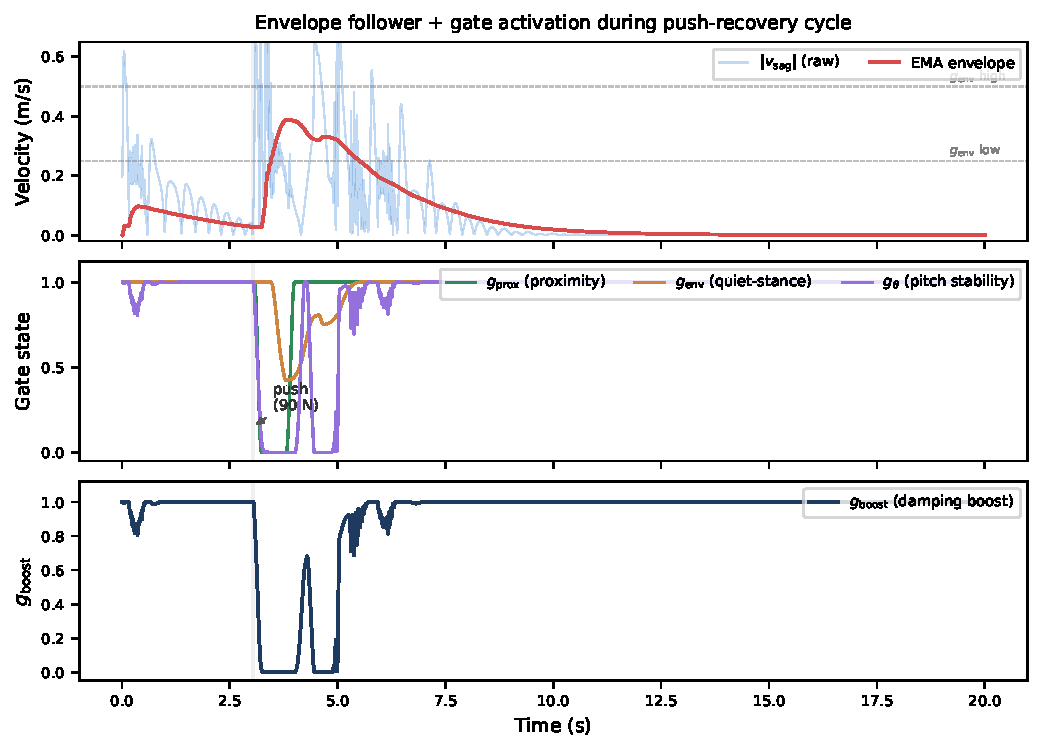
\includegraphics[width=\linewidth]{figures/gate_activation.pdf}
    \caption{Gate activation during a \SI{90}{N} lateral (world $+x$) push-recovery cycle (\SI{100}{Hz} control). \textbf{Top:} $|v_{\text{sag}}|$ and asymmetric EMA envelope; dashed lines mark the \SIrange{0.25}{0.50}{m/s} quiet-stance band. \textbf{Middle:} Individual gate states. \textbf{Bottom:} Composite damping boost $g_{\text{boost}}$. Grey shading: \num{7}-step push window. The three panels are the empirical basis for finding (iii) of \S\ref{sec:idle_mechanism}: $g_{\text{prox}}$ and $g_{\text{env}}$ both sit pinned at their quiet-stance values before the impulse and after the ringdown, which is why ablating either reproduces ACC bit-for-bit at idle, and why only a disturbance experiment can measure their contribution.}
    \label{fig:gate_activation}
\end{figure*}

\subsection{Posture and Yaw Stability ($\boldsymbol{\tau}_{\text{posture}}$)}
\label{sec:posture}

Posture regulation uses Jacobian-based PD gains scheduled across 23 heights:

\begin{equation}
\begin{split}
\boldsymbol{\tau}_{\text{posture}} =\;&
\boldsymbol{\tau}_{\text{PD}}^{\text{jac}}(q,\dot{q},h^{\text{cmd}})
+ \boldsymbol{\tau}_{\text{div}}(q_{\text{hy}}^L,q_{\text{hy}}^R)\\
&+ g_{\text{settled}}\,\boldsymbol{\tau}_{\text{homing}}(q-q_{\text{ref}}),
\end{split}
\label{eq:posture}
\end{equation}

where $\boldsymbol{\tau}_{\text{div}}$ damps hip-yaw divergence and $\boldsymbol{\tau}_{\text{homing}}$ restores nominal posture when upright and settled.
Yaw return uses wheel-differential torque.

\subsection{Contact-Loss Recovery ($g_{\text{flight}}\!\cdot\!\boldsymbol{\tau}_{\text{flight}}$)}
\label{sec:flight}

When both wheels lose ground contact, ACC detects this via per-wheel normal forces and substitutes a flight attitude controller using the wheels as reaction flywheels:

\begin{align}
g_{\text{flight}} &= \begin{cases}
1, & \text{if } F_z^L, F_z^R < 0.5mg \text{ for } {\geq} 2 \text{ steps},\\
0, & \text{if } \min(F_z^L,F_z^R) \geq 0.5mg \text{ for } {\geq} 5 \text{ steps},
\end{cases}\\[2pt]
\boldsymbol{\tau}_{\text{flight}} &= \operatorname{clip}\!\big(2.0\theta + 0.5\dot{\theta} - 0.02\omega_{\text{wheel}},\;\pm\SI{2}{Nm}\big).
\label{eq:flight}
\end{align}

Forward wheel spin pitches nose-up during descent; \num{5}-step release
hysteresis prevents balance-torque re-engagement during bounce. The free-fall
drop is a stress test and the ledge drive-off the intended use case. We note in
advance of the results that this override is the one ACC mechanism whose
ablation does \emph{not} show it to be necessary at the reported scales: the
wheel--inverted-pendulum loop it replaces is itself a reaction-flywheel
controller when the wheels are unloaded, and the override's measured
contribution is to bound landing-attitude variance near the upper end of the
drop envelope rather than to enable recovery (\S\ref{sec:flight_terrain_results},
Table~\ref{tab:flight_ext}).

\subsection{Per-Leg Ground Adaptation ($g_{\text{terrain}}$)}
\label{sec:terrain}

When the two wheels rest at different ground heights---a curb straddle, an
oblique ledge---a single torso height command forces the torso to roll by the
step angle. ACC instead maintains an \emph{independent ground estimate per leg}
and issues two height commands. The estimate is taken from the wheel
contact-point height, which is exact at any body tilt for a rigid wheel, and is
updated only while that wheel carries real load:
\begin{equation}
\hat{h}_{\text{gnd}}^{i} \leftarrow \hat{h}_{\text{gnd}}^{i}
+ \alpha_g\big(z_{\text{contact}}^{i} - \hat{h}_{\text{gnd}}^{i}\big),
\quad F_z^{i} \geq 0.2mg, \quad i \in \{L,R\},
\label{eq:terrain_est}
\end{equation}
with $\alpha_g = 0.35$ per control step to reject contact chatter. The
$0.2mg$ load test rather than mere geometric touching is deliberate: a lightly
touching wheel that is in the act of unloading rides a few centimetres high and
injected a \SI{+2.9}{cm} phantom ground step on the \SI{15}{cm} curb.

An unloaded wheel does \emph{not} update~\eqref{eq:terrain_est}. It freezes its
estimate, because an airborne wheel supplies no information about where its
ground is. The one exception is the only physically unambiguous
``my ground is gone'' signal---the wheel centre descending \emph{below} its own
believed ground:
\begin{equation}
\delta^{i} > \SI{3}{mm}
\;\Rightarrow\;
\dot{\hat{h}}_{\text{gnd}}^{i} = -\big(v_0 + k_s \,\delta^{i}\big),
\label{eq:terrain_seek}
\end{equation}
where $\delta^{i} = \hat{h}_{\text{gnd}}^{i} - z_{\text{contact}}^{i}$ is the
depth by which the wheel has fallen below its believed ground,
with $v_0 = \SI{0.5}{m/s}$ and $k_s = \SI{50}{\per\second}$. The
proportional term matters: a fixed slew converged the ground estimate in
\SI{0.30}{s}, by which time a \SI{20}{cm} dismount had already tipped the robot
past recovery, whereas a \SI{15}{cm} drop under~\eqref{eq:terrain_seek} slews at
\SI{8}{m/s} and converges within two control steps, so the leg extends
\emph{during} the fall rather than after it. When both wheels are airborne, both
estimates track the mean wheel height, which reproduces the symmetric
pre-adapter behaviour exactly and leaves ballistic flight to
\S\ref{sec:flight}.

The step $\Delta h = \hat{h}_{\text{gnd}}^{L} - \hat{h}_{\text{gnd}}^{R}$ is
then absorbed by the legs rather than the torso. The split is kinematic, not a
linear height offset: with $L(\cdot)$ the forward-kinematic leg length and
$L^{-1}$ its inverse over the calibrated posture range, the leg on the higher
ground is shortened by the full step,
\begin{align}
L_{\text{high}} &= L\big(h^{\text{cmd}}\big) - |\Delta h|,\\
h^{\text{high}} &= L^{-1}\!\big(L_{\text{high}}\big), \qquad
h^{\text{low}} = h^{\text{cmd}},
\label{eq:terrain_split}
\end{align}
both clamped to the calibrated envelope extended by \SI{10}{cm} at each end. To
first order this is the familiar $h^{\text{cmd}} \mp \Delta h/2$ symmetric
split, but the $h \mapsto L$ map is markedly nonlinear near full squat: the
linear proxy erred by \SI{12}{cm} at the lower extrapolation limit, folding the
knee back under the thigh. If $L_{\text{high}}$ falls below the shortest
physically reachable leg, ACC raises the \emph{whole} robot until the short leg
fits, trading commanded height for the ability to span the step. A
\SI{20}{cm} curb at nominal stance exceeds even this: it would require
\SI{170}{\degree} of knee flexion against a \SI{2.7}{rad} limit, and the
uncompensated remainder appears as a predicted torso roll
$\arctan(-\varepsilon / w_{\text{track}})$ with $\varepsilon$ the unspanned
step and $w_{\text{track}} = \SI{0.278}{m}$ the wheel separation. Reporting
this expected roll explicitly is what keeps a legitimate straddle from being
misread as an incipient fall by the tilt-based safety monitors.

Because the $h \mapsto L$ table is itself extrapolated at the extremes, a
purely feedforward split left a systematic \SI{+6}{\degree} torso roll on the
\SI{10}{cm} curb. A closed-loop leveling integrator trims the split by the
\emph{measured} roll at \SI{0.15}{m/(rad.s)} with \SI{\pm 6}{cm} of authority.
It integrates only when all three of the following hold: both wheels loaded, a
genuine ground step $|\Delta h| \geq \SI{2}{cm}$, and a ground estimate settling
at less than \SI{0.15}{m/s}. The gating is not cosmetic. Without the step
condition, the dynamic roll of a turn is integrated as if it were terrain and
wound an \SI{8.6}{\degree} roll bias through a \SI{180}{\degree} turn; without
the rate condition, the geometric transient of a curb climb is integrated as a
leveling error and compresses the flat leg. Off-step, the trim decays to zero
with a \SI{1}{s} time constant.

% Platform comparison table — qualitative, not binary
\begin{table}[t]
\centering
\footnotesize
\caption{Capability comparison across wheeled biped platforms. ``---'' = not reported in cited work. Idle precision and push force are not standardized benchmarks; quantitative cross-platform comparison is limited by metric heterogeneity.}
\label{tab:platform_comparison}
\setlength{\tabcolsep}{2pt}\begin{tabular}{@{}>{\raggedright\arraybackslash}p{1.3cm}>{\raggedright\arraybackslash}p{1.1cm}>{\raggedright\arraybackslash}p{1.1cm}>{\raggedright\arraybackslash}p{1.1cm}>{\raggedright\arraybackslash}p{1.1cm}>{\raggedright\arraybackslash}p{1.85cm}@{}}
\toprule
Metric & Ascento & DIABLO & Whleaper & SKATER & \textbf{ACC (Ours)} \\
\midrule
Balance &
  LQR &
  Cascaded\newline LQR &
  LQR + PPO &
  Convex\newline MPC &
  \textbf{Gated PD\newline + anchor I} \\
\midrule
Idle precision &
  --- &
  --- &
  --- &
  --- &
  \textbf{\SI{0.294}{mm}\newline sag.\ CoM RMS} \\
\midrule
Push recovery &
  ---\textsuperscript{a} &
  --- &
  --- &
  --- &
  \textbf{8-dir.,}\newline $F_{\text{med}}{=}$\,\SI{117}{N} \\
\midrule
Height &
  Discrete\newline jump &
  Stance\textsuperscript{b} &
  Multi-modal &
  Contin. &
  \textbf{\SIrange{0.35}{0.45}{m}}\newline CoM\textsuperscript{c} \\
\midrule
Flight &
  Jumping\newline (airtime) &
  --- &
  --- &
  --- &
  \textbf{Drop \SI{100}{cm},\newline ledge \SI{50}{cm}} \\
\midrule
Terrain &
  --- &
  --- &
  --- &
  Vision-based &
  \textbf{Per-leg\newline contact} \\
\midrule
\textbf{Validation} &
  Hardware &
  Hardware &
  Hardware &
  Hardware &
  \textbf{Simulation} \\
\bottomrule
\end{tabular}
\vspace{2pt}\tabnote\noindent
\textsuperscript{a}Qual.\ omnidirectional push recovery demonstrated in supplementary video; quantitative force thresholds not reported in cited work.
\textsuperscript{b}Height variation demonstrated; quantitative range not reported.
\tabnote\noindent
\textsuperscript{c}Calibrated CoM-$z$ band (\S\ref{sec:height_convention}), $\pm\SI{5}{cm}$ about the \SI{0.404}{m} nominal, with joint targets extrapolated to \SIrange{0.254}{0.554}{m}; commanded $\pm\SI{5}{cm}$ transitions are evaluated under disturbance in \S\ref{sec:analysis}. Not comparable to the base-$z$ ranges of the cited platforms or of our PPO baseline.
\end{table}

\subsection{Complete Numerical Parameter Set}
\label{sec:parameters}

Table~\ref{tab:parameters} lists core parameters; the full set (50+ gains) is available in the supplementary material.

\begin{table}[t]
\centering
\footnotesize
\caption{Core numerical parameters for the ACC balance controller. All values in SI units unless noted otherwise.}
\label{tab:parameters}
\begin{tabular}{@{}p{2.8cm}rp{1.8cm}@{}}
\toprule
\multicolumn{3}{c}{\textbf{Balance Core}} \\
\midrule
$k_p$                      & 50      & Nm/rad \\
$k_d$                      & 3.0     & Nm/(rad/s) \\
$k_{\text{pos}}$           & 20      & Nm/m \\
Position clip              & $\pm$4.0 & Nm \\
$k_{\text{vel}}$           & 15      & Nm/(m/s) \\
Vel.\ damp.\ scale         & 1.5     & --- \\
$k_{\text{roll}}$          & 55      & Nm/rad \\
$k_{\text{roll},d}$        & 5.5     & Nm/(rad/s) \\
$k_{\text{yaw}}$           & 1.0     & Nm/rad \\
$k_{\text{yaw},d}$         & 0.3     & Nm/(rad/s) \\
$k_{\text{pos,return}}$    & 2.0     & Nm/m \\
$k_{\text{heading}}$       & 2.0     & Nm/rad \\
$k_{\text{heading},d}$     & 0.6     & Nm/(rad/s) \\
\midrule
\multicolumn{3}{c}{\textbf{Anchor Mechanism}} \\
\midrule
$K_i$ (anchor integral)    & 4.0     & Nm/(m$\cdot$s) \\
Integral cap               & 2.0     & Nm \\
Integral leak              & 5$\times$10$^{-3}$ & per step \\
Boost scale $k_{\text{vb}}$& 5.0     & --- \\
$g_{\text{prox}}$ band     & 0.05--0.15 & m \\
$g_{\text{env}}$ band      & 0.25--0.50 & m/s \\
$\tau_{\text{attack}}$     & 0.023   & s \\
$\tau_{\text{release}}$    & 1.5     & s \\
$g_{\text{stab}}$ ($\theta$) & 2--12  & $^\circ$ \\
$g_{\text{stab}}$ ($\dot{\theta}$) & 2--15 & $^\circ$/s \\
\midrule
\multicolumn{3}{c}{\textbf{Flight / Terrain / Other}} \\
\midrule
$k_{\text{flight}}$ (P / D)& 2.0 / 0.5 & --- \\
Wheel damping (flight)     & 0.02    & Nm/(rad/s) \\
Flight engage / release    & 2 / 5   & steps \\
\makecell[l]{$F_z$ thresh.\\(flight / terrain)} & 0.5 / 0.2 & $\times mg$ \\
\bottomrule
\end{tabular}
\vspace{2pt}\tabnote\noindent
\end{table}

% ============================================================
\section{Experimental Validation}
\label{sec:results}
% ============================================================

We evaluate ACC across four scenario classes, each mapped to the component it tests and paired with targeted ablations.
ACC is evaluated at \SI{500}{Hz} simulation / \SI{100}{Hz} control; the PPO and LQR baselines run at \SI{50}{Hz}, their own design rate. All configurations use a \SI{400}{Nm/s} torque rate limit per joint.

\emph{Control rate.} Because ACC's headline comparison is against controllers designed for a slower loop, we do not rely on the design-rate numbers alone: every classical baseline is additionally re-run at ACC's \SI{100}{Hz} under an otherwise identical protocol, holding episode length fixed in seconds rather than in steps. The rate-matched results are reported in \S\ref{sec:rate_matched} (Table~\ref{tab:rate_matched}) and show that doubling the baselines' rate does not change the outcome. The converse direction---ACC at \SI{50}{Hz}---is a negative result: with the discrete coefficients recomputed for the longer step ($\alpha_a{\approx}0.58$ and $\alpha_r{\approx}0.013$, re-derived from Eq.~\eqref{eq:asym_ema} at $\Delta t{=}\SI{0.02}{s}$, with the anchor leak rescaled to \num{0.010} per step) the controller is not preserved. The robot collapses, and the mean CoM height over the recorded window is \SI{0.124}{m} against a nominal standing height of \SI{0.404}{m}. The $\SI{0.050}{mm}$ ``idle RMS'' and the \SI{10}{N} push threshold produced by that run are artifacts of a robot lying motionless on the ground---\SI{10}{N} is the lower bound of the binary search, returned when even the smallest tested impulse fails. We therefore report \emph{no} \SI{50}{Hz} ACC result and make no claim that the architecture is rate-independent downward; this is analysed as Limitation~5.
RNG seeds are deterministic: idle standing uses $\text{seed} = 20260727 + \text{trial\_id}$; push ablation uses $\text{seed} = 20260728 \times 100 + \text{rep}$; LQR baselines cycle seeds $\{0, 42, 123\}$ across episodes.

\subsection{Anchored Standing}
\label{sec:standing}

\subsubsection{Two precision metrics, deliberately kept separate}

``Standing precision'' names two different quantities in the wheeled-biped
literature, and they are not interchangeable. Let $\mathbf{p}(t)\in\mathbb{R}^2$ be
the horizontal base position over an evaluation window of length $T$, let
$\mathbf{p}_0$ be the commanded home position, and let
$\bar{\mathbf{p}}=\frac{1}{T}\int_0^T\mathbf{p}(t)\,dt$ be the trial mean. We report

\begin{align}
A &= \Bigl(\tfrac{1}{T}\textstyle\int_0^T \lVert\mathbf{p}(t)-\mathbf{p}_0\rVert^2\,dt\Bigr)^{1/2},
\label{eq:accuracy}\\
R &= \Bigl(\tfrac{1}{T}\textstyle\int_0^T \lVert\mathbf{p}(t)-\bar{\mathbf{p}}\rVert^2\,dt\Bigr)^{1/2}.
\label{eq:repeatability}
\end{align}

$A$ is the \emph{accuracy}: RMS displacement from the position the controller was
told to hold. It retains any DC parking offset, so it answers ``how close to the
commanded pose does the robot actually park?''. $R$ is the \emph{repeatability}:
RMS about the trial's own mean, with the DC offset removed. It answers ``how still
is the robot once it has parked?''. A controller with a persistent \SI{27}{mm}
offset and a perfectly steady hold scores $A{=}\SI{27}{mm}$ but
$R{\approx}\SI{0}{mm}$; a controller centred on the target but oscillating scores
the reverse. Reporting either alone is uninformative, and---because the two differ
by more than an order of magnitude on this platform---comparing a value of one
against a value of the other produces a meaningless ratio.

Both are reported for every configuration below, resolved separately along the
sagittal axis, the lateral axis, and the full plane, because the two horizontal
axes of this platform are not merely different in degree---they are actuated by
different means and must not be pooled or interchanged. We therefore fix the
convention explicitly, since the two are easy to transpose and the physical
conclusions invert if they are:

\begin{itemize}
\item The \textbf{sagittal} axis is world $y$. Both wheel axles point along world
$x$ and the two wheels are separated along world $x$
($w_{\text{track}}{=}\SI{0.278}{m}$), so the rolling direction---the axis on
which wheel torque produces ground force, and the only axis with a genuine
inverted-pendulum mode---is world $y$. The controller agrees: \verb|init_v3_controller|
packs $\hat{\mathbf{s}}=(0,1)$ as its sagittal unit vector.
\item The \textbf{lateral} axis is world $x$. No actuator produces lateral ground
force; the axis is held passively by the wheel contacts and by the roll restoring
moment of the track width.
\end{itemize}

\noindent Two dynamic checks confirm the assignment rather than merely asserting
it. A \SI{90}{N} impulse along $y$ is absorbed with a peak wheel speed of
\SI{52}{rad/s} and leaves a residual offset of \SI{4.8}{mm}---the wheels drive
back under the CoM---whereas the same impulse along $x$ leaves a permanent
\SI{23.2}{mm} offset at a peak wheel speed of \SI{18}{rad/s}, because nothing can
push the robot sideways again. And over a \SI{20}{s} quiet stance the robot rolls
\SI{24.6}{mm} along $y$ with the wheel midpoint tracking the CoM to within
\SI{0.2}{mm}, while $x$ holds to \SI{0.02}{mm}. All four checks are reproduced by
\texttt{scripts/verify\_body\_axes.py}, which asserts on disagreement.

This matters for reading Table~\ref{tab:standing}: the anchor integral and the
gated damping boost both live in the wheel-torque channel, so \emph{both act on
the sagittal axis only}. The lateral column is therefore a measure of how little
the plant moves when nothing drives it, not a measure of controller quality, and
the sagittal and planar columns carry essentially all of the information about
what ACC does (Sec.~\ref{sec:discussion}, Limitation~8).

\subsubsection{Unified measurement protocol}

Every row of Table~\ref{tab:standing} was re-measured under one protocol so that no
two entries in the same column come from different definitions.
Each trial runs \SI{25}{s} at \SI{500}{Hz} physics / \SI{100}{Hz} control from the
nominal standing pose with randomized initial conditions
($\sigma{=}\SI{0.005}{rad}$ per joint, clipped to joint limits;
$\sigma{=}\SI{1}{mm}$ on root height), seeded
$\text{seed}{=}20260727{+}\text{trial\_id}$ for $\text{trial\_id}\in[0,10)$.
The first \SI{5}{s} are discarded as settling---long enough to cover the
EMA$_0{=}0$ transient (${\sim}\SI{7.5}{s}$ to full release, but ${<}\SI{5}{s}$ to
within \SI{1}{\percent} of the quiet-stance value)---and $A$ and $R$ are computed
over the remaining \SI{20}{s}. Displacements are taken relative to each trial's own
$t{=}0$ pose, so $\mathbf{p}_0$ is the commanded home rather than the world origin.
A trial is scored as a fall if $|\theta|{>}\SI{46}{\degree}$ or root height
${<}\SI{0.15}{m}$ at any point. Confidence intervals are Student-$t$
($t_{9,0.025}{=}2.262$, $\text{SEM}{=}\text{SD}/\sqrt{10}$).

We note explicitly what this protocol \emph{cannot} test: because every trial starts
at the commanded home, it never exercises the anchor's return-to-home function. It
measures the controller's ability to \emph{stay} put, not to \emph{come back}. The
latter is measured by the push experiments of Sec.~\ref{sec:push}. This distinction
turns out to matter for attributing the mechanism (Sec.~\ref{sec:idle_mechanism}).

\begin{table*}[t]
\centering
\caption{Idle standing precision across the full ablation ladder. All rows re-measured under the single protocol of Sec.~\ref{sec:standing}; values are mean${\pm}$SD over $N{=}10$ trials. See the note below the table for column definitions.}
\label{tab:standing}
\setlength{\tabcolsep}{5pt}
\begin{tabular}{@{}ll S[table-format=2.3(4)] S[table-format=2.3(3)] S[table-format=2.3(4)] S[table-format=-2.1] S[table-format=2.3(4)] c@{}}
\toprule
& \multirow{2}{*}{Configuration}
& {$R_{\text{sag}}$ (mm)} & {$R_{xy}$ (mm)} & {$R_{\text{lat}}$ (mm)} & {$\bar{s}$ (mm)} & {$A_{\text{lat}}$ (mm)} & Survival \\
& & {sagittal rep.} & {planar rep.} & {lateral rep.} & {sag.\ offset} & {lateral acc.} & \\
\midrule
\multicolumn{8}{@{}l}{\textbf{Additive ladder (bottom-up)}}\\
L0   & P-only (PD, no position, no integral) & 17.461(258) & 17.845(279) & 3.675(246) & -44.8 & 9.933(712) & 10/10 \\
L1   & $+$ position homing ($\pm\SI{0.10}{m}$) & 20.397(17) & 20.414(19) & 0.834(66) & -30.4 & 2.629(884) & 10/10 \\
L2   & $+$ ungated integral $K_i$ & 25.026(39) & 25.056(43) & 1.212(110) & -27.5 & 3.661(1264) & 10/10 \\
L2.5 & $+$ proximity gate only (no envelope, no boost) & 25.198(17) & 25.227(20) & 1.205(99) & -27.6 & 4.023(1194) & 10/10 \\
\midrule
\multicolumn{8}{@{}l}{\textbf{Proposed controller}}\\
L3/S1 & \textbf{ACC} (full anchor, fixed $k_p{=}50$) & \bfseries 0.294(15) & \bfseries 0.788(69) & \bfseries 0.730(73) & \bfseries -27.0 & \bfseries 1.213(554) & \textbf{10/10} \\
\midrule
\multicolumn{8}{@{}l}{\textbf{Subtractive ablation (top-down from ACC)}}\\
S0 & ACC $+$ scheduled $k_p$ (rejected variant) & 0.294(15) & 0.788(69) & 0.730(73) & -27.0 & 1.213(554) & 10/10 \\
S2 & $-$ gated damping boost & 4.772(69) & 4.824(67) & 0.703(69) & -26.8 & 1.260(616) & 10/10 \\
S3 & $-$ asymmetric envelope (symmetric EMA) & 0.294(15) & 0.788(69) & 0.730(73) & -27.0 & 1.213(554) & 10/10 \\
S4 & $-$ proximity gate (integral always on) & 0.294(15) & 0.788(69) & 0.730(73) & -27.0 & 1.213(554) & 10/10 \\
S5 & $-$ pitch safety gate $g_\theta$ & {---} & {---} & {---} & {---} & {---} & \textbf{0/10} \\
\midrule
\multicolumn{8}{@{}l}{\textbf{Single-mechanism isolation (ACC with one term disabled)}}\\
M1 & $K_i{=}0$ (anchor integral removed, gates intact) & 0.089(35) & 0.733(72) & 0.727(71) & -31.2 & 1.192(535) & 10/10 \\
M2 & damping terms reverted to their L2 values & 25.198(17) & 25.227(20) & 1.205(99) & -27.6 & 4.023(1194) & 10/10 \\
M3 & $K_i{=}0$ \emph{and} boost $=0$ & 3.973(130) & 4.037(128) & 0.710(69) & -31.1 & 1.241(591) & 10/10 \\
\bottomrule
\end{tabular}
\vspace{2pt}\tabnote\noindent
\textbf{Protocol.} $N{=}10$ trials, \SI{100}{Hz} control, \SI{20}{s} measurement
window after a \SI{5}{s} settle, clean sensors, \SI{0}{ms} actuator delay.

\noindent\textbf{Columns.} $R$ = repeatability (RMS about the trial mean,
Eq.~\eqref{eq:repeatability}); $A$ = accuracy (RMS from commanded home,
Eq.~\eqref{eq:accuracy}); $\bar{s}$ = mean signed sagittal parking offset.
Sagittal is world $y$ and lateral is world $x$ (Sec.~\ref{sec:standing}). The
anchor integral and the damping boost act on the sagittal axis only, so
$R_{\text{sag}}$ and $\bar{s}$ are the columns that discriminate between
configurations, while $R_{\text{lat}}$ measures a passively held axis and is
near-constant by construction.

\noindent\textbf{Omitted columns.} $A_{\text{sag}}$ and $A_{xy}$ carry no
information beyond the columns shown: over all twelve surviving rows the
identities $A_{\text{sag}}=\sqrt{\bar{s}^{2}+R_{\text{sag}}^{2}}$ and
$A_{xy}=\sqrt{A_{\text{sag}}^{2}+A_{\text{lat}}^{2}}$ hold to \SI{0.003}{mm}
and \SI{0.02}{mm} respectively---accuracy on an axis is just that axis's
parking offset and its repeatability added in quadrature.

\noindent Produced by \path{scripts/collect_idle_ladder.py} (per-trial worker
\path{scripts/_idle_ladder_worker.py}); raw output
\path{outputs/paper_verification/idle_ladder.json}.
\end{table*}

\subsubsection{Result}

ACC holds \textbf{sub-millimeter sagittal repeatability},
$R_{\text{sag}} = 0.294{\pm}\SI{0.015}{mm}$ (95\%\,CI $[0.283,0.305]$\,mm), across
ten randomized trials with no falls. This is the figure of merit for the platform,
because sagittal is the actuated inverted-pendulum axis: it is the axis on which
the robot can fall, the axis the wheel-torque channel drives, and the axis that
every configuration in the ladder is trying to hold.

We deliberately do not quote a signal-to-noise ratio against a simulator noise
floor here. The floor is measured by locking the joints and pinning the base
(\path{run_r2_between_trial_stats.py --noise-floor}), and that procedure only
zeroes velocities rather than welding the base, so it is trustworthy on the
laterally-constrained axis (\SI{0.0019}{mm} RMS) but not on the gravity-loaded
sagittal and vertical axes, where the residual sag it reports
(\SI{5.79}{mm} and \SI{63.5}{mm}) is an artifact of the pinning rather than
integrator noise. The relevant scale for $R_{\text{sag}}$ is instead the spread
\emph{between} configurations measured under the identical protocol: removing a
single mechanism (S2) moves $R_{\text{sag}}$ from \num{0.294} to \SI{4.772}{mm},
a factor of \num{16} with non-overlapping SDs, which is what establishes that the
metric resolves the effect being studied.

Against the P-only baseline (L0), which sustains the \SI{69.7}{mm} peak-to-peak
sagittal limit cycle described in Sec.~\ref{sec:intro}, the like-for-like
improvements are

\begin{itemize}
\item sagittal repeatability $R_{\text{sag}}$: $17.461 \rightarrow \SI{0.294}{mm}$, a factor of \textbf{59.4};
\item planar repeatability $R_{xy}$: $17.845 \rightarrow \SI{0.788}{mm}$, a factor of \textbf{22.6};
\item lateral repeatability $R_{\text{lat}}$: $3.675 \rightarrow \SI{0.730}{mm}$, a factor of \textbf{5.0}.
\end{itemize}

The ordering of these three factors is itself informative and worth stating
plainly, because it is the opposite of what a reader might expect. The largest
gain is on the sagittal axis, which is the hard axis; the smallest is on the
lateral axis, which is the easy one. That is the correct signature for a
wheel-torque controller: every term ACC adds beyond L0---position homing, the
anchor integral, the gated damping boost---produces ground force along the
rolling direction and none of them can produce lateral force at all. The residual
$5{\times}$ lateral improvement is an indirect consequence of the robot pitching
and yawing less, not of any lateral control action, and we do not claim it as one.
A reader comparing against platforms that report a single scalar ``standing
precision'' should compare against $R_{\text{sag}}$, not against
$R_{\text{lat}}$ or a planar norm, since the latter two are diluted by an axis
this class of platform does not actuate.

\emph{The accuracy picture is markedly worse than the repeatability picture, and
on the same axis.} ACC parks $\bar{s}={-}\SI{27.0}{mm}$ from the commanded home
along the sagittal axis and holds that offset to within \SI{0.009}{mm} SD across
trials---the robot rolls backwards by \SI{27}{mm} during the settle and then stands
there, exceptionally still, in the wrong place. Planar accuracy is therefore
$A_{xy}=\SI{26.994}{mm}$ and improves only $1.8{\times}$ over L0
($49.1\rightarrow\SI{27.0}{mm}$), a full order of magnitude worse than the
repeatability gain. The offset is not a measurement artifact and not an
unregulated axis: it lies precisely on the axis the anchor integral does control,
and the integral reduces it only from \SI{31.2}{mm} (M1, $K_i{=}0$) to
\SI{27.0}{mm}. An ideal integrator would drive it to zero. We report the
discrepancy as the principal open weakness of the present design (Limitation~8)
rather than absorbing it into a planar average where it is less visible.

\subsubsection{Which mechanism produces the precision}
\label{sec:idle_mechanism}

The bottom two blocks of Table~\ref{tab:standing} isolate the contributions. Four
findings are worth stating precisely, because three of them contradict the
attribution that the gate structure invites.

\emph{(i) Idle steadiness comes from the damping ladder; the integral buys
accuracy instead.} The two contributions separate cleanly once the axes are kept
apart, and they do not compete for the same metric.

M1 disables the anchor integral entirely ($K_i{=}0$) while leaving every gate in
place, and its \emph{repeatability} is not merely as good as ACC's but slightly
better ($R_{\text{sag}}$ \SI{0.089}{mm} vs.\ ACC's \SI{0.294}{mm};
$R_{xy}$ \SI{0.733}{mm} vs.\ \SI{0.788}{mm}). Its \emph{accuracy}, however, is
worse by \SI{4.2}{mm}: it parks at $\bar{s}={-}\SI{31.2}{mm}$ against ACC's
$-\SI{27.0}{mm}$. That is the integral's entire measurable idle signature, and it
is exactly the trade one expects from an integral term---it walks the robot
closer to the commanded home at the cost of a small amount of steadiness, since
the accumulating term is itself a slowly-varying command. A protocol that reports
repeatability alone will conclude, wrongly, that the anchor integral is inert at
idle; a protocol that reports accuracy alone will miss that it costs a factor of
three in steadiness.

Conversely M2 keeps the integral and every gate but reverts the two
velocity-damping coefficients to their L2 values, and reproduces the L2/L2.5 limit
cycle exactly ($R_{\text{sag}}=\SI{25.198}{mm}$). Steadiness is therefore
attributable to the damping terms, in two stages: raising the velocity-damping
scale takes $R_{\text{sag}}$ from \SI{25.2}{mm} to \SI{3.97}{mm} (M3, boost still
off), and enabling the gated damping boost takes it from \SI{3.97}{mm} to
\SI{0.294}{mm} (ACC)---a combined factor of \num{86} decomposed into factors of
${\sim}\num{6.3}$ and ${\sim}\num{13.5}$. S2 confirms the second stage
independently from the top down: removing only the boost degrades
$R_{\text{sag}}$ from \SI{0.294}{mm} to \SI{4.772}{mm}.

\emph{(ii) The damping boost acts sagittally, as it must.} S2 degrades sagittal
repeatability by a factor of \num{16} ($0.294\rightarrow\SI{4.772}{mm}$) while
leaving lateral repeatability statistically unchanged
($R_{\text{lat}}=\SI{0.703}{mm}$ vs.\ ACC's \SI{0.730}{mm}, overlapping CIs). This
is the only outcome consistent with the architecture: the boost multiplies a
velocity-damping coefficient inside the wheel-torque channel
(Eq.~\eqref{eq:balance}), and wheel torque generates ground force along the
rolling direction only. The residual oscillation it suppresses is therefore a
sagittal pitching/rolling-forward mode, and an evaluation that reported the
lateral axis alone would conclude, wrongly, that the boost does nothing at idle.
We flag this explicitly because the lateral column is the one that looks like a
plausible ``$x$-axis RMS'' to report by default, and it is the one column in
Table~\ref{tab:standing} that is nearly blind to every mechanism in the ladder:
across all twelve surviving configurations $R_{\text{lat}}$ spans only
\SIrange{0.70}{3.68}{mm}, and across the seven rows that retain the full damping
ladder (S0--S4, M1, M3) only \SIrange{0.70}{0.73}{mm}.

\emph{(iii) The proximity gate and the asymmetric envelope are inert during quiet
stance.} S4 (proximity gate removed) and S3 (symmetric envelope) are
\emph{bit-identical} to ACC on every idle metric. This is the expected behavior
rather than a null result: during quiet stance the base never leaves the \SI{5}{cm}
inner band, so $g_{\text{prox}}{\equiv}1$ and gating it changes nothing; and the
velocity envelope never rises into the attack branch, so the asymmetric and symmetric
followers produce the same signal. Both mechanisms are defined by what they do when
the robot is \emph{displaced}---windup prevention during a push (S4) and ringdown
after one (S3)---and are correctly evaluated only in Table~\ref{tab:push_ablation}.
The idle protocol, which starts at home and stays there, is blind to both by
construction.

\emph{(iv) The pitch safety gate is required even to stand.} S5 falls in
\num{10}/\num{10} trials during pure quiet stance, with no push applied. Removing
$g_\theta$ leaves the damping boost free to act on the pitch state at large
excursions, and the resulting positive feedback diverges from the ${\pm}\SI{0.005}{rad}$
initial perturbation alone. This is a stronger safety result than the push-only
evidence previously reported for this ablation.

Taken together: the anchor's \emph{gates} are what make an aggressive damping and
integral configuration admissible without windup or divergence, while the damping
terms they admit are what deliver the steadiness. The gates are enabling
conditions, not the proximate cause of the precision---a distinction the earlier
framing of this work conflated. The integral's primary role is drift rejection
under disturbance, which by construction cannot appear in a protocol that starts
at the target; its measurable idle signature is confined to the \SI{4.2}{mm}
reduction in sagittal parking offset noted above (M1 $-31.2$ vs.\ ACC
$\SI{-27.0}{mm}$), bought at a $3{\times}$ cost in sagittal repeatability. Both
effects sit on the sagittal axis, and neither is visible on the lateral one.

Post-push velocity ringdown decays within \SI{9}{s} under ACC, whereas P-only
oscillates indefinitely because the \SI{1.3}{Nm} equilibrium bias sustains the limit
cycle. The symmetric-EMA ablation exhibits bistable failure: a post-push cycle holds
the envelope at ${\approx}0.10$, leaving the boost gate half-open, and the robot
oscillates perpetually. The ungated-integral ablation winds up during the push and
prevents recovery entirely. All three of these are post-push behaviors and are
quantified in Sec.~\ref{sec:push}.

\subsection{Omnidirectional Push Recovery}
\label{sec:push}

Push recovery is evaluated via polar sweep: \SIrange{10}{160}{N} impulses (\num{7} control steps) at the torso in \num{8} directions.
Bearings are applied in the world frame as $\mathbf{f}=F(\cos\theta,\sin\theta,0)$, so $\theta{=}\pm\SI{90}{\degree}$ are the sagittal (fore/aft) bearings and $\theta{=}\SI{0}{\degree}/\SI{180}{\degree}$ the lateral ones, per the axis convention of Sec.~\ref{sec:standing}.
$F_{\min}$ is the maximum magnitude survived in \emph{every} direction; $F_{\text{med}}$ is the median.
All thresholds measured via binary search over $[\SI{10}{N},\SI{160}{N}]$ (\num{8} iterations per direction, \SI{5}{N} tolerance).
Survival: torso pitch $<\SI{46}{\degree}$ for \SI{17}{s} post-push.

\emph{Single-bearing stress tests.} Several auxiliary experiments in this paper---the robustness sweep (Table~\ref{tab:robustness}), the rate-limit sweep, the ringdown and gate-activation traces (Figs.~\ref{fig:gate_activation},~\ref{fig:ringdown}), and the compound-disturbance protocol (Table~\ref{tab:compound})---apply a single impulse along world $+x$ rather than repeating the full \num{8}-bearing sweep, which would multiply their cost eightfold. That bearing is \emph{lateral}, and it is a below-median one: the polar sweep places $\SI{0}{\degree}$ at $\SI{94.3}{N}$, third-weakest of the eight and \SI{22.6}{N} below $F_{\text{med}}$. Those experiments are therefore conservative probes of ACC's disturbance margin, not optimistic ones, and we label them as lateral throughout rather than as ``forward.'' The omnidirectional figures ($F_{\min}$, $F_{\text{med}}$) are the ones that characterize the full envelope.

\begin{table}[t]
\centering
\footnotesize
\caption{Factorial ablation of ACC components: push-recovery and ringdown metrics. Clean sensors, all rows $N{=}10$, mean${\pm}$std. See the note below the table for definitions and significance tests.}
\label{tab:push_ablation}
\setlength{\tabcolsep}{5pt}\begin{tabular}{@{}c>{\raggedright\arraybackslash}p{3.1cm}rr>{\raggedright\arraybackslash}p{1.5cm}@{}}
\toprule
& Configuration & $F_{\min}$ (N) & $F_{\text{med}}$ (N) & Ringdown \\
\midrule
\multicolumn{5}{@{}l}{\textbf{Additive (bottom-up)}} \\
\midrule
L0 & P-only (PD, no pos., no I)  & 70.0${\pm}$1.0 & 122.1${\pm}$2.1 & never \\
L1 & $+$\,Pos.\ homing ($\pm$\SI{0.10}{m}) & 74.8${\pm}$0.8 & 130.5${\pm}$1.2 & never \\
L2 & $+$\,Integral $K_i$ (no gate) & 76.1${\pm}$1.1 & 132.0${\pm}$2.0 & --- \\
L2.5 & $+$\,Prox.\ gate only (no EMA, no boost) & 75.5${\pm}$0.9 & 132.0${\pm}$2.3 & --- \\
L3 & $+$\,Full anchor (gate, EMA, boost)\textsuperscript{7} & \bfseries 82.8${\pm}$1.0 & 116.8${\pm}$4.7 & \textbf{\SI{9.0}{s}} \\
\midrule
\multicolumn{5}{@{}l}{\textbf{Subtractive (top-down from ACC)}} \\
\midrule
S0 & ACC $+$ scheduled $k_p$ (rejected)\textsuperscript{6}  & 79.4${\pm}$2.6 & 114.0${\pm}$5.3 & \SI{9.0}{s} \\
S1 & \textbf{ACC}\textsuperscript{6} (canonical, fixed $k_p{=}50$) & \bfseries 82.8${\pm}$1.0 & 116.8${\pm}$4.7 & \textbf{\SI{9.0}{s}} \\
S2 & $-$Damping boost           & 84.2${\pm}$1.1 & 115.5${\pm}$5.3 & never\textsuperscript{1} \\
S3 & $-$Asym.\ EMA (sym.\ EMA)  & 81.6${\pm}$2.3 & 109.2${\pm}$5.4 & never\textsuperscript{2} \\
S4 & $-$Prox.\ gate (global I)  & 80.0${\pm}$2.5 & 114.0${\pm}$5.3 & windup\textsuperscript{3} \\
S5 & $-$Pitch gate $g_\theta$   & 8.8${\pm}$0.6\textsuperscript{5} & 35.4${\pm}$10.3 & never\textsuperscript{4} \\
\bottomrule
\end{tabular}
\vspace{2pt}\tabnote\noindent
$F_{\min}$ and $F_{\text{med}}$ are the minimum and median survivable push over \num{8} bearings, each located by binary search to \SI{5}{N} tolerance. Idle-precision metrics for these same configurations are reported separately in Table~\ref{tab:standing} under a single measurement protocol; they are deliberately not duplicated here, because idle and push behaviour are governed by different subsets of the gates.\tabnote\noindent
\textsuperscript{1}Boost necessary for ringdown.
\textsuperscript{2}Symmetric EMA bistable: post-push oscillation holds EMA in mid-band.
\textsuperscript{3}Without the proximity gate the integral accumulates throughout the displacement and saturates its cap; the robot survives the impulse but does not settle. At idle this ablation is bit-identical to ACC (Table~\ref{tab:standing}), since the base never leaves the gate's inner band.
\textsuperscript{4}Removing the pitch gate lets the damping boost act on the pitch state at large excursions; the resulting parametric amplification diverges. This ablation additionally fails \num{10}/\num{10} at pure idle with no push applied (Table~\ref{tab:standing}).
\textsuperscript{5}Below measurement floor (\SI{10}{N}); robot cannot survive minimal push.
\textsuperscript{6}S1 (fixed $k_p{=}50$) is the canonical ACC configuration. S0 (scheduled $k_p$, softened from 50 to 35 during pushes) was tested and rejected---it did not improve push survival.
\textsuperscript{7}L2$\rightarrow$L3 = canonical ACC (S1, fixed $k_p{=}50$); bundles four mechanisms (prox.\ gate, asym.\ EMA, boost, pitch gate). S2--S5 isolates each subtractively.
Welch's unpaired $t$-test (two-sided, $N{=}10$ per group, independent trials; Welch--Satterthwaite $\text{df}{\in}[9,18]$; uncorrected $p$, Bonferroni-adj.\ $\alpha{=}0.007$, see \S\ref{sec:discussion}): L0$\rightarrow$L1 $+$\SI{4.8}{N} ($p{<}0.001$); L1$\rightarrow$L2 $+$\SI{1.3}{N} (n.s.); L2$\rightarrow$L2.5 $-$\SI{0.6}{N} (n.s., gate alone adds nothing); L2.5$\rightarrow$L3 $+$\SI{7.3}{N} ($p{<}0.001$). S5 (pitch gate) is critical to safety ($F_{\min}{=}\SI{8.8}{N}$, and \num{0}/\num{10} survival even at idle); S2 and S3 are required for ringdown. Idle metrics for every row are in Table~\ref{tab:standing}. With $N{=}10$, 95\%CI half-width ${\approx}0.72{\times}$std ($t_{0.025,9}{=}2.262$, single-group $\text{df}{=}9$); sub-\SI{2}{N} differences (e.g., S1 vs.\ S3 $\Delta F_{\min}{=}\SI{1.2}{N}$, CI$_{95}$(S1)${\approx}{\pm}\SI{0.7}{N}$, CI$_{95}$(S3)${\approx}{\pm}\SI{1.6}{N}$) remain non-significant. Produced by \path{scripts/replicate_ablation_n10.py}. Raw outputs: rows L2 and S0--S5 in \path{outputs/paper_statistics/ablation_n10_results.json}; row L2.5 in \path{outputs/paper_statistics/ablation_n10_L2_5.json}; rows L0 and L1 in \path{outputs/paper_statistics/push_ci_all_ablations.json}. All at $N{=}10$ under the same protocol.
\end{table}

Table~\ref{tab:push_ablation} reports the factorial ablation.
Additively: L1 (homing) adds \SI{4.8}{N} over L0 ($p{<}0.001$); L2 (global integral) adds only \SI{1.3}{N} over L1 (n.s.); L3 (full anchor) adds \SI{6.7}{N} over L2 ($p{<}0.001$). The L2$\rightarrow$L3 step bundles four mechanisms at once, and the push metrics alone cannot separate them; Sec.~\ref{sec:idle_mechanism} performs that separation on the idle side. What the push data do show is that the proximity gate contributes nothing to push \emph{margin} on its own (L2$\rightarrow$L2.5, $-\SI{0.6}{N}$, n.s.), consistent with its role being windup prevention rather than capture-basin enlargement, and that the full anchor recovers a margin advantage over the ungated integral ($+\SI{6.7}{N}$) while simultaneously being the only configuration in the ladder that settles.
Subtractively: S1 (fixed $k_p{=}50$, canonical) matches or exceeds S0 in all metrics, confirming gain scheduling is unnecessary---the anchor and boost alone resolve the trade-off. The gated damping boost (S2) is the dominant idle-precision mechanism, and it acts sagittally: removing it degrades sagittal repeatability sixteen-fold (\SI{0.294}{mm}${\rightarrow}\SI{4.772}{mm}$) while leaving lateral repeatability statistically unchanged (\SI{0.703}{mm} vs.\ ACC's \SI{0.730}{mm}, Table~\ref{tab:standing}). Its push margin is, if anything, slightly better without the boost ($F_{\min}=\SI{84.2}{N}$ vs.\ \SI{82.8}{N}), so the boost buys sagittal steadiness and settling, not capture basin. S5 (pitch gate) is critical to safety---removing it collapses $F_{\min}$ to $8.8{\pm}0.6$\,N (${\sim}9{\times}$ below ACC) and additionally causes \num{10}/\num{10} falls at pure idle. S3 (asymmetric EMA) and S2 are each individually required for ringdown.

\begin{figure}[t]
    \centering
    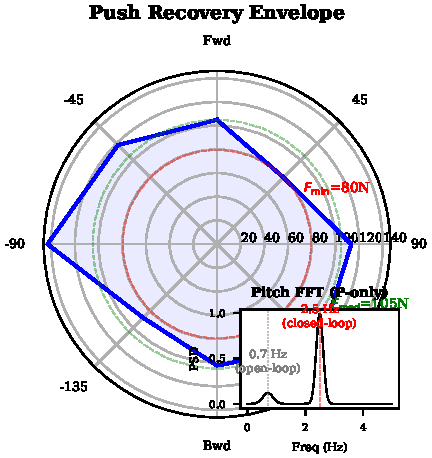
\includegraphics[width=\linewidth]{figures/polar_push_envelope.pdf}
    \caption{Omnidirectional push envelope of ACC. This is the \emph{same} run
    as row S1 of Table~\ref{tab:push_ablation}, not a separate measurement:
    \num{8} bearings, $N{=}\num{10}$ repetitions each, threshold located by
    binary search over \SIrange{10}{160}{N} to a \SI{5}{N} tolerance, so the
    plotted minimum is by construction the $F_{\min}$ of that row. Solid curve:
    per-bearing mean survivable push magnitude; shaded band: ${\pm}1$ standard
    deviation over the ten repetitions. The radial axis is linear in force and
    originates at \SI{0}{N}, so radial distance is proportional to margin.
    The envelope is strongly anisotropic, spanning
    \SIrange{82.8}{142.7}{N}---a $1.7{\times}$ ratio between the weakest and
    strongest bearing. The ordering is
    $-\SI{90}{\degree}\,(\SI{142.7}{N}) >
      \SI{135}{\degree}\,(\SI{132.9}{N}) >
      \SI{90}{\degree}\,(\SI{120.9}{N}) >
      -\SI{45}{\degree}\,(\SI{118.0}{N}) >
      \SI{180}{\degree}\,(\SI{100.7}{N}) >
      \SI{0}{\degree}\,(\SI{94.3}{N}) >
      -\SI{135}{\degree}\,(\SI{93.1}{N}) >
      \SI{45}{\degree}\,(\SI{82.8}{N})$.
    Two regularities are visible. First, the actuated axis is the strong one:
    bearings are applied in the world frame as
    $\mathbf{f}=F(\cos\theta,\sin\theta,0)$, so $\pm\SI{90}{\degree}$ are purely
    sagittal and $\SI{0}{\degree}/\SI{180}{\degree}$ purely lateral
    (Sec.~\ref{sec:standing}). The two sagittal bearings average \SI{131.8}{N}
    against \SI{97.5}{N} for the two lateral ones, a $1.35{\times}$ advantage.
    This is the expected asymmetry for a wheeled biped: sagittally the wheels
    accelerate the contact patch back under the CoM and convert the impulse into
    a controlled excursion, whereas laterally no actuator produces ground force
    at all and the only restoring authority is the static
    $w_{\text{track}}={\SI{0.278}{m}}$ track width plus hip-roll PD. We compare
    axis \emph{means} rather than ranks because the raw ordering is contaminated
    by the second regularity. Second, the envelope is
    measurably \emph{chiral}: $\SI{135}{\degree}$ survives \SI{40}{N} more than
    $-\SI{135}{\degree}$, and $-\SI{90}{\degree}$ \SI{22}{N} more than
    $\SI{90}{\degree}$. An independent earlier sweep of a neighbouring
    configuration reproduces both asymmetries with the same sign and comparable
    magnitude, so this is a systematic property of the plant-plus-controller
    rather than sampling noise; we have not isolated its origin, and it is
    reported here as an observation rather than an explained effect
    (Sec.~\ref{sec:discussion}). $F_{\min}$ (red) is the bearing-wise minimum
    and is the figure of merit quoted throughout the paper, because it is the
    magnitude survived in \emph{every} direction; $F_{\max}$ (blue) is shown
    only to indicate the spread.}
    \label{fig:push_polar}
\end{figure}

\begin{figure}[t]
    \centering
    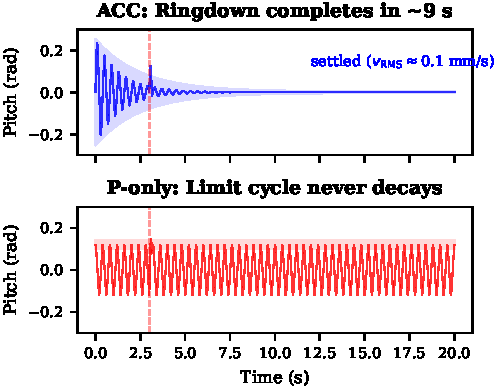
\includegraphics[width=\linewidth]{figures/ringdown_time_series.pdf}
    \caption{Post-push recovery (\SI{90}{N} lateral, world $+x$, at $t{=}\SI{3}{s}$). \textbf{Top:} attitude angles; stabilization within \SI{2}{s}. \textbf{Bottom:} planar CoM position, which separates the two axes cleanly. The lateral push couples through roll into a large \emph{sagittal} excursion (\SI{-251}{mm} peak); the anchor drives that axis back to $\SI{+1.37}{mm}$ of home and holds it there at \SI{0.018}{mm} SD over the final \SI{2}{s}---a \SI{99.5}{\percent} recovery. On the pushed lateral axis, which has no actuator authority (Sec.~\ref{sec:standing}), the \SI{200}{mm} peak excursion decays only to a permanent $\SI{+36.2}{mm}$ offset, \SI{18}{\percent} of the peak. The contrast between the two traces is the clearest single illustration of what the anchor does and where it does not act.}
    \label{fig:ringdown}
\end{figure}

\subsection{Flight Recovery and Terrain Adaptation}
\label{sec:flight_terrain_results}

ACC's two-channel assembly supports independent extensions without modifying the core anchor. Both extensions use the same \SI{400}{Nm/s} rate limit and \SI{100}{Hz} control rate.

\emph{Contact-loss recovery.}
ACC recovers to a settled stand from a \SI{100}{cm} free drop (10/10,
$24.0{\pm}1.2^\circ$ peak pitch after touchdown) and from a \SI{50}{cm} ledge
drive-off (10/10, $27.1{\pm}2.0^\circ$ peak landing pitch); the \SI{60}{cm} drop
and \SI{20}{cm} ledge are correspondingly milder (Table~\ref{tab:flight_ext}).
The two flight ablations, however, give a more nuanced picture than the
mechanism's design rationale suggests, and we report it as measured.

Removing the flight \emph{attitude} PD (the reaction-flywheel term
$2.0\theta + 0.5\dot\theta$, spin-down damping retained) is a real but modest
loss: peak pitch rises from $24.0$ to $\SI{27.8}{\degree}$ on the \SI{100}{cm}
drop with one fall in ten, and from $27.1$ to $\SI{31.6}{\degree}$ on the
\SI{50}{cm} ledge with no falls. Removing the airborne wheel-torque override
\emph{entirely}---so the ordinary wheel--inverted-pendulum (WIP) loop keeps
driving the wheels through flight---does not degrade either condition at all: it
\emph{lowers} peak pitch to $13.0{\pm}\SI{0.5}{\degree}$ (drop) and
$10.2{\pm}\SI{0.4}{\degree}$ (ledge) at 10/10 survival, because free wheels
driven by the pitch-feedback loop are themselves an effective reaction flywheel.
The override's benefit appears only at the upper end of the envelope: at
\SI{150}{cm} the two configurations survive equally (2/5 settled either way) but
the override holds peak pitch to $34.0{\pm}\SI{2.1}{\degree}$ against
$53.6{\pm}\SI{35.0}{\degree}$ without it---a \num{16}$\times$ reduction in
spread, with one uncontrolled trial exceeding \SI{90}{\degree}. At \SI{200}{cm}
both configurations fail. The correct claim is therefore that the flight override
\textbf{bounds landing-attitude variance near the envelope limit}, not that it
enables the recovery; at the \SIrange{50}{100}{cm} scales reported here ACC's
balance core alone suffices. We state this explicitly because the mechanism was
originally introduced to prevent a nose-down crash observed in an earlier
controller revision, and that failure mode is no longer reachable in the present
design.

\emph{Per-leg terrain adaptation.}
Here the ablation is unambiguous. With per-leg adaptation, straddle roll on the
one-wheel curb is $2.5{\pm}\SI{0.04}{\degree}$ (\SI{10}{cm}),
$3.5{\pm}\SI{3.2}{\degree}$ (\SI{15}{cm}) and $14.9{\pm}\SI{0.1}{\degree}$
(\SI{20}{cm}), all 10/10. Replacing \texttt{split()} with a symmetric posture
(both legs commanded to the same height---the pre-adapter behaviour) causes a
fall at \emph{every} tested curb height, \num{0}/\num{10} in all three cases:
the torso rolls past \SI{60}{\degree} within \SI{0.8}{s} of curb entry and the
robot is on the ground by \SI{2.3}{s}. The height split is thus load-bearing for
this task in a way the flight override is not. The closed-loop leveling trim that
rides on top of the split is a second-order refinement of the same mechanism:
disabling it alone leaves the robot upright on the \SI{10}{cm} curb
($3.2{\pm}\SI{0.08}{\degree}$, 10/10) but degrades the \SI{15}{cm} curb to
$11.1{\pm}\SI{1.6}{\degree}$ roll with \num{6}/\num{10} settled---the trim
corrects the residual error of the non-linear height$\rightarrow$leg-length
table, which grows with step height.
At \SI{20}{cm} the limit is one of joint authority, not of the split geometry.
Evaluating~\eqref{eq:terrain_split} at $h^{\text{cmd}}{=}\SI{0.404}{m}$ gives
commanded leg lengths of \SI{0.350}{m} (flat) and \SI{0.150}{m} (curb), i.e.\ a
difference equal to the full \SI{20}{cm} step with \emph{zero} kinematic
residual---the posture pair can span the curb exactly. What tightens is the
joint budget: the compressed leg's commanded knee angle grows
\SI{2.18}{rad}~(\SI{10}{cm}) $\rightarrow$ \SI{2.39}{rad}~(\SI{15}{cm})
$\rightarrow$ \SI{2.58}{rad}~(\SI{20}{cm}) against a hard limit of
\SI{2.70}{rad}, leaving only \SI{0.12}{rad} (\SI{6.6}{\degree}) of headroom, and
the commanded CoM height of that leg, \SI{0.265}{m}, sits within \SI{1.1}{cm} of
the extrapolation floor $z_{\text{lo}}{-}\SI{10}{cm}{=}\SI{0.254}{m}$.
Because the commanded posture is exact, the measured \SI{14.9}{\degree} straddle roll
is entirely \emph{tracking} error: in this deeply flexed configuration the leg
carries its load at the shortest gravitational moment arm the PID gains were
never re-tuned for, and it settles below its target. Adaptation therefore still
prevents leg-fold (\num{10}/\num{10} survival), but the torso is left tilted; the
tight $\pm\SI{0.1}{\degree}$ std reflects a deterministic, saturation-dominated
equilibrium rather than genuinely low run-to-run variability.

\begin{table}[t]
\centering
\caption{Contact-loss recovery and per-leg terrain adaptation, with the
corresponding mechanism ablations. All at \SI{400}{Nm/s} rate limit,
\SI{100}{Hz} control. Survival is the \emph{strict settle} verdict (flat
pitch/roll window, tail height error ${\leq}\SI{12}{mm}$, residual speed
${\leq}\SI{0.05}{m/s}$), not merely staying upright.}
\label{tab:flight_ext}
\footnotesize
\setlength{\tabcolsep}{4pt}
\begin{tabular}{@{}>{\raggedright\arraybackslash}p{3.5cm}rrr@{}}
\toprule
\multicolumn{4}{c}{\textbf{Contact-Loss Recovery}} \\
\midrule
Scenario / ablation & $N$ & Peak Pitch ($^\circ$) & Settled \\
\midrule
Drop \SI{100}{cm}    & 10 & 24.0$\pm$1.2 & 10/10 \\
Drop \SI{60}{cm}     & 10 & 18.2$\pm$1.0 & 10/10 \\
Ledge \SI{50}{cm}    & 10 & 27.1$\pm$2.0 & 10/10 \\
Ledge \SI{20}{cm}    & 10 & 19.6$\pm$0.3 & 10/10 \\
\addlinespace[1pt]
$-$Attitude PD, drop \SI{100}{cm}\textsuperscript{a}   & 10 & 27.8$\pm$0.3 & 9/10 \\
$-$Attitude PD, ledge \SI{50}{cm}\textsuperscript{a}   & 10 & 31.6$\pm$2.2 & 10/10 \\
$-$Flight override, drop \SI{100}{cm}\textsuperscript{b} & 10 & 13.0$\pm$0.5 & 10/10 \\
$-$Flight override, ledge \SI{50}{cm}\textsuperscript{b} & 10 & 10.2$\pm$0.4 & 10/10 \\
\addlinespace[1pt]
Drop \SI{150}{cm} (envelope edge)      & 5 & 34.0$\pm$2.1 & 2/5 \\
$-$Flight override, drop \SI{150}{cm}\textsuperscript{b} & 5 & 53.6$\pm$35.0 & 2/5 \\
\midrule
\multicolumn{4}{c}{\textbf{Per-Leg Terrain (One-Wheel Curb, \SI{0.15}{m/s})}} \\
\midrule
Configuration & $N$ & Straddle Roll ($^\circ$) & Settled \\
\midrule
Full adaptation, \SI{10}{cm}  & 10 & 2.5$\pm$0.04 & 10/10 \\
Full adaptation, \SI{15}{cm}  & 10 & 3.5$\pm$3.2 & 10/10 \\
Full adaptation, \SI{20}{cm}  & 10 & 14.9$\pm$0.1 & 10/10 \\
\addlinespace[1pt]
$-$Leveling trim, \SI{10}{cm}\textsuperscript{c} & 10 & 3.2$\pm$0.08 & 10/10 \\
$-$Leveling trim, \SI{15}{cm}\textsuperscript{c} & 10 & 11.1$\pm$1.6 & 6/10 \\
\addlinespace[1pt]
$-$Height split, \SI{10}{cm}\textsuperscript{d} & 10 & \multicolumn{1}{c}{fall} & 0/10 \\
$-$Height split, \SI{15}{cm}\textsuperscript{d} & 10 & \multicolumn{1}{c}{fall} & 0/10 \\
$-$Height split, \SI{20}{cm}\textsuperscript{d} & 10 & \multicolumn{1}{c}{fall} & 0/10 \\
\bottomrule
\end{tabular}
\vspace{2pt}\tabnote\noindent
$\pm$std over $N$ trials with randomized ICs ($\pm\SI{0.003}{rad}$ joint,
$\pm\SI{1.5}{mm}$ CoM). Drop metric: peak $|\theta|$ from touchdown onward;
ledge metric: peak $|\theta|$ through landing; curb metric: max $|\phi|$ while
straddling the curb top.
\textsuperscript{a}Reaction-flywheel attitude PD zeroed; airborne spin-down damping retained.
\textsuperscript{b}Entire airborne wheel-torque override bypassed---the ordinary WIP loop drives the wheels through flight.
\textsuperscript{c}Closed-loop leveling integrator disabled; per-leg height split retained.
\textsuperscript{d}\texttt{split()} forced to a symmetric posture (both legs at the same commanded height), i.e.\ pre-adapter behaviour; roll diverges past \SI{60}{\degree} within \SI{0.8}{s} of curb entry, so no straddle-roll statistic exists.
\tabnote\noindent
Produced by \path{scripts/collect_flight_terrain_n10.py}; raw output
\path{outputs/flight_terrain_n10/results.json}.
\end{table}

The gate structure isolates each extension to its physical regime without
re-tuning the anchor, and both extensions cost three lines of controller code
each. Their measured \emph{necessity}, however, differs sharply: the per-leg
height split is required for the curb task at every tested height, whereas the
flight override is a variance-bounding refinement that only pays at the top of
the drop envelope.

\begin{figure}[t]
    \centering
    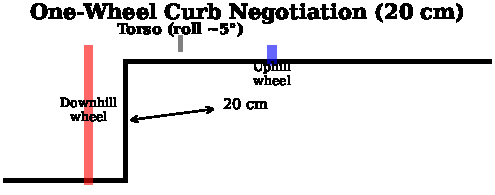
\includegraphics[width=\linewidth]{figures/curb_straddle.pdf}
    \caption{One-wheel curb (\SI{20}{cm}). With the per-leg height split:
    $14.9{\pm}0.1^\circ$ straddle roll, 10/10 settled. With a symmetric posture
    (split removed): the curb-side leg cannot fold far enough, roll diverges
    past \SI{60}{\degree} within \SI{0.8}{s} of curb entry, 0/10.}
    \label{fig:curb}
\end{figure}

\subsection{Comparison with Classical and Learning-Based Baselines}
\label{sec:baselines}

To establish ACC is not merely a tuned linear controller or un-structured policy, we compare seven baselines---six classical (four 4-state TWIP variants: LQR, LQR+AW, LQR-DT, PI+AW; two 6-state coupled variants: servo and direct-torque) plus a preliminary PPO baseline (all share identical environment setups):

\begin{enumerate}
\item \textbf{LQR}---4-state TWIP with decoupled roll/yaw PD through a PID servo layer ($\sim$\SI{0.25}{s} lag).
\item \textbf{LQR + Integral AW}---Same as (1) plus pitch-error integral with conditional AW (clamped $\pm\SI{3.0}{rad/s}$).
\item \textbf{LQR (Direct Torque)}---Re-optimized for direct-torque plant ($\tau_s{=}0$, $k_{p,\text{roll}}{=}55.0$), outputting torques directly.
\item \textbf{Coupled 6-State 3D LQR}---Extends (1) with roll states $(\phi,\dot{\phi})$.
\item \textbf{PI + AW (Direct Torque)}---DT-LQR $+$ integral AW on fwd.\ position (conditional, $\pm\SI{15}{cm}$ gate); same leg/roll/yaw as DT-LQR.
\item \textbf{Pure PPO (Preliminary)}---Model-free RL policy trained from scratch for \num{5.4}M environment steps (single seed, in \texttt{BalanceEnv}).
\item \textbf{Coupled 6-State LQR (Direct Torque)}---Same 6-state model as (4) but outputs direct torques (bypassing PID servo, $\sim$\SI{0.25}{s} lag removed). Gains re-derived for the direct-torque plant ($K_{\text{pitch}}{=}113$, $K_{\text{roll}}{=}58$\,Nm/rad); leg posture via PD position control.
\end{enumerate}

Direct-torque LQR removes the servo path, eliminating both the PID gains and the measured actuation lag. PI+AW adds integral anti-windup on forward position to DT-LQR---the standard engineering fix for a DC position bias, with windup protection. The anti-windup logic is verified independently by \texttt{scripts/validate\_lqr\_aw.py}. PPO evaluates what unconstrained model-free policy search achieves on the same plant. Every gain used for these seven baselines is listed in Table~\ref{tab:baseline_gains}; we give them in full because the central claim of this subsection is a \emph{negative} one---that no member of this family stands---and a negative result is only as strong as the tuning behind it.

\begin{table}[t]
\centering
\footnotesize
\caption{Baseline gain derivation. All weights follow Bryson's rule; see the note below the table.}
\label{tab:baseline_gains}
\setlength{\tabcolsep}{4pt}
\begin{tabular}{@{}>{\raggedright\arraybackslash}p{1.75cm}>{\raggedright\arraybackslash}p{6.15cm}@{}}
\toprule
Controller & Gains and derivation \\
\midrule
LQR (4-state) & $Q{=}\operatorname{diag}(10,2,3,0.3)$, $R{=}0.8$; roll and yaw closed by decoupled PD through the PID servo layer \\
\addlinespace[2pt]
LQR $+$ AW & as above, plus a pitch-error integral with conditional anti-windup, clamped to $\pm\SI{3.0}{rad/s}$ \\
\addlinespace[2pt]
LQR, DT & 4-state gains re-optimized for the zero-lag plant: $\tau_s{=}0$, $k_{p,\text{roll}}{=}55.0$ \\
\addlinespace[2pt]
6-state LQR & $Q{=}\operatorname{diag}(10,2,3,0.5,3,0.3)$, $R{=}\operatorname{diag}(0.8,1.0)$, derived in continuous time and shared by the servo and DT variants \\
\addlinespace[2pt]
6-state LQR, DT & state feedback re-solved for the zero-lag plant: $K_{\text{pitch}}{=}113$, $K_{\text{roll}}{=}\SI{58}{Nm/rad}$ (see Limitation~7) \\
\addlinespace[2pt]
PI $+$ AW, DT & DT-LQR gains plus an integral on forward position: $k_{i,\text{pos}}{=}\SI{8.0}{rad/s/(m{\cdot}s)}$, clamp $\pm\SI{5.0}{rad/s}$, conditional gate $\pm\SI{15}{cm}$ \\
\midrule
PID servo layer & $k_p{=}[55,40,70,70,4]$, $k_d{=}[3,2,4,4,0]$, $k_i{=}[0.8,0.4,1,1,0.1]$, ordered (hip roll, hip yaw, hip pitch, knee, wheel) \\
\addlinespace[2pt]
Servo lag & \SI{0.25}{s}, measured as the wheel-velocity \SI{90}{\percent} rise time ($\approx\num{25}$ steps at \SI{100}{Hz}) \\
\bottomrule
\end{tabular}
\vspace{2pt}\tabnote\noindent\footnotesize
Bryson's rule throughout ($Q_{ii}{=}1/x_{i,\max}^{2}$, $R{=}1/u_{\max}^{2}$); the \num{46}-configuration retuning sweep described in the text confirmed that no retuning within these ranges changes the outcome. The 4-state model is (pitch, pitch-rate, forward velocity, forward position); the 6-state model adds (roll, roll-rate). ``DT'' denotes direct torque, i.e.\ the PID servo path removed and $\tau_s{=}0$.
\end{table}

\begin{table}[t]
\centering
\footnotesize
\caption{LQR and PPO baselines vs.\ ACC, clean sensors. Parenthesised $N$ is the episode count. See the note below the table.}
\label{tab:lqr_baselines}
\setlength{\tabcolsep}{4pt}
\begin{tabular}{@{}l S[table-format=2.2] S[table-format=1.3] S[table-format=2.2] S[table-format=3.1] S[table-format=2.2]@{}}
\toprule
Configuration & {Surv.} & {$\theta_{\text{RMS}}$} & {$\phi_{\text{RMS}}$} & {$H_{\text{RMS}}$} & {$\tau_{\text{RMS}}$} \\
& {(s)} & {(\si{\degree})} & {(\si{\degree})} & {(mm)} & {(Nm)} \\
\midrule
LQR, TWIP ($N{=}60$)         & 0.52 & 0.04  & 24.2 & 371.0 & 92.10 \\
LQR $+$ AW ($N{=}60$)        & 0.52 & 0.04  & 24.2 & 371.0 & 92.10 \\
LQR, DT (re-opt.) ($N{=}20$) & 0.72 & 0.78  & 21.2 & 135.0 & 9.33 \\
6-St.\ LQR ($N{=}20$)        & 0.52 & 0.04  & 24.2 & 371.0 & 92.10 \\
PI $+$ AW, DT ($N{=}20$)     & 0.72 & 0.78  & 21.2 & 135.0 & 9.33 \\
6-St.\ LQR, DT ($N{=}20$)    & 0.16 & 0.00  & 21.1 & 117.0 & 13.90 \\
Pure PPO (prelim.) ($N{=}20$)& 3.20 & 4.82  & 3.15 & 54.2  & 18.40 \\
\midrule
\textbf{ACC} ($N{=}10$)      & \bfseries 20.00 & \bfseries 0.060 & \bfseries 0.010 & \bfseries 0.18 & \bfseries 3.28 \\
\bottomrule
\end{tabular}
\vspace{3pt}\tabnote\noindent\footnotesize
LQR / LQR+AW / 6-St.\ use the PID servo; LQR (DT), PI+AW (DT) and 6-St.\ (DT) command torque directly; PPO is a 5.4M-step RL policy (preliminary, single seed). The identical LQR / LQR+AW / 6-St.\ rows arise because all three saturate at the common \SI{30}{Nm} limit through the same PID servo within \SI{0.52}{s}, masking the gain differential.\tabnote\noindent
Between-episode standard deviations (omitted above for legibility):
LQR / LQR$+$AW / 6-St.: $\pm0.00$, $\pm0.01$, $\pm2.1$, $\pm45$, $\pm3.2$;
LQR-DT / PI$+$AW-DT: $\pm0.00$, $\pm0.42$, $\pm0.3$, $\pm41$, $\pm1.18$;
6-St.\ DT: $\pm0.00$ on every metric (deterministic failure);
PPO: $\pm0.85$, $\pm0.91$, $\pm0.45$, $\pm8.3$, $\pm2.1$;
ACC: $\pm0.00$, $\pm0.006$, $\pm0.001$, $\pm0.02$, $\pm0.00$.
\vspace{2pt}\tabnote\noindent All LQR and PI+AW variants fall within \SI{0.72}{s} (\SI{100}{\percent}); the 6-St.\ DT variant falls deterministically at \SI{0.16}{s} (zero trial-to-trial variance, $N{=}20$), confirming that removing the servo path with gains derived from a simplified model does not rescue stability. PI+AW (DT-LQR $+$ integral AW on fwd.\ position) yields metrics identical to DT-LQR: the integral cannot accumulate before roll-induced fall at $\sim$\SI{0.72}{s}. Preliminary PPO achieves partial standing but suffers \SI{85}{\percent} falls over multi-height transitions ($H_{\text{RMS}}{=}\SI{54.2}{mm}$). $N{=}60$ for LQR/LQR+AW (sweep); $N{=}20$ for DT/6-St./PI+AW/6-St.\ DT/PPO.
\end{table}

Table~\ref{tab:lqr_baselines} reports the comparison.
All six classical baselines---four derived from the 4-state TWIP model (LQR, LQR+AW, LQR-DT, PI+AW) and two 6-state coupled variants (servo, direct-torque)---fall within \SI{0.72}{s}. Removing the PID servo path (4-state DT-LQR: $\tau_s{=}0$, $k_{p,\text{roll}}{=}55.0$, no integral) reduces torque \num{10}$\times$ (\SI{92.1}{Nm} $\rightarrow$ \SI{9.33}{Nm}) and marginally improves roll ($\phi_{\text{RMS}}{=}\SI{21.2}{\degree}$ vs.\ \SI{24.2}{\degree}). Adding a forward-position integral (PI+AW: $k_{i,\text{pos}}{=}8.0$, conditional $\pm\SI{15}{cm}$ gate) changes nothing---the integral cannot accumulate before the roll-induced fall at \SI{0.72}{s}---confirming the 4-state TWIP model is structurally insufficient for this articulated-leg platform.
Preliminary PPO (5.4M steps, single seed) sustains single-height standing longer (\SI{3.20}{s}) but exhibits an \SI{85}{\percent} fall rate across multi-height command transitions (\SI{54.2}{mm} height error).
ACC achieves $0.060{\pm}0.006^\circ$ pitch RMS, $0.010{\pm}0.001^\circ$ roll RMS, $0.18{\pm}0.02$\,mm CoM Z, and $3.28{\pm}0.00$\,Nm torque RMS ($N{=}10$).
A \textbf{46-configuration} sweep (dimensions as given in Table~\ref{tab:baseline_gains}; script \path{scripts/sweep_lqr_roll_gains.py}) confirmed all tested LQR variants fail (\SI{100}{\percent}); a 6-state coupled LQR with direct torque actuation, removing the PID servo path, also fails---indicating platform complexity, not servo lag alone, is the dominant factor (see Limitation~7).
Neither servo-lag removal nor preliminary PPO training (5.4M steps, single seed) resolved the height-adaptive posture trade-off in our experiments; whether a fully converged PPO policy closes this gap is not tested here.

\subsubsection{Removing the control-rate confound}
\label{sec:rate_matched}

Table~\ref{tab:lqr_baselines} compares controllers running at different rates: ACC at \SI{100}{Hz} and every classical baseline at \SI{50}{Hz}, its design rate. Taken alone this leaves ACC a $2{\times}$ control-bandwidth advantage, and a reader is entitled to ask whether that advantage, rather than the architecture, produces the gap. We removed the confound in the direction that can actually be measured---by raising the baselines to \SI{100}{Hz} rather than lowering ACC to \SI{50}{Hz}---and report the result in Table~\ref{tab:rate_matched}.

\begin{table}[t]
\centering
\footnotesize
\caption{Rate-matched baselines: every classical controller re-run at ACC's \SI{100}{Hz}. Physics is \SI{500}{Hz} throughout; only the substeps per control step change. See the note below the table.}
\label{tab:rate_matched}
\setlength{\tabcolsep}{2.2pt}
\begin{tabular}{@{}l S[table-format=1.2] S[table-format=2.2] S[table-format=2.2] S[table-format=2.2] S[table-format=3.1] S[table-format=3.1]@{}}
\toprule
& \multicolumn{2}{c}{Surv.\ (s)} & \multicolumn{2}{c}{$\phi_{\text{RMS}}$ (\si{\degree})} & \multicolumn{2}{c}{$H_{\text{RMS}}$ (mm)} \\
\cmidrule(lr){2-3}\cmidrule(lr){4-5}\cmidrule(lr){6-7}
Configuration & {\SI{50}{Hz}} & {\SI{100}{Hz}} & {\SI{50}{Hz}} & {\SI{100}{Hz}} & {\SI{50}{Hz}} & {\SI{100}{Hz}} \\
\midrule
LQR, TWIP        & 0.52 & 0.32 & 24.21 & 24.21 & 370.6 & 205.8 \\
LQR $+$ AW       & 0.52 & 0.32 & 24.19 & 24.21 & 370.7 & 205.8 \\
LQR, DT          & 0.72 & 0.60 & 21.22 & 27.48 & 135.0 & 119.2 \\
6-St.\ LQR       & 0.52 & 0.32 & 24.20 & 24.21 & 370.6 & 205.8 \\
PI $+$ AW, DT    & 0.72 & 0.52 & 21.22 & 26.14 & 135.0 & 171.3 \\
6-St.\ LQR, DT   & 0.16 & 0.16 & 21.05 & 21.19 & 117.2 & 128.5 \\
\midrule
\textbf{ACC}     & {---} & \bfseries 20.00 & {---} & \bfseries 0.010 & {---} & \bfseries 0.18 \\
\bottomrule
\end{tabular}
\vspace{3pt}\tabnote\noindent\footnotesize
\textbf{Protocol.} $N{=}20$ episodes per cell, seeds $\{0,42,123\}$, nominal scenario, clean sensors, \SI{0}{ms} actuator delay. Episode length is held fixed in \emph{seconds}, not steps: \num{1000} steps at \SI{50}{Hz} and \num{2000} steps at \SI{100}{Hz} both cover \SI{20}{s}. The LQR feedback gains are continuous-time and therefore rate-independent; the rate change affects only the substep count, the drift and integral accumulators, the torque rate limiter, and (for the FD-linearized variant) the linearization step.\tabnote\noindent
\textbf{Outcome.} Fall rate is \SI{100}{\percent} in all twelve baseline cells. The \SI{50}{Hz} columns reproduce Table~\ref{tab:lqr_baselines}: survival time matches exactly on all six rows and $\phi_{\text{RMS}}$ matches at that table's one-decimal precision, with residual differences of ${\le}\SI{0.4}{mm}$ in $H_{\text{RMS}}$ and ${\le}\SI{0.04}{Nm}$ in $\tau_{\text{RMS}}$ (the two servo rows are quoted there at $N{=}60$ rather than the $N{=}20$ used here). This validates the rate-matched harness against the original measurement, so the \SI{100}{Hz} columns differ from the \SI{50}{Hz} ones only by the intended change. ACC is shown at \SI{100}{Hz} only; the \SI{50}{Hz} ACC run is analysed as a negative result in Limitation~5 and is not a usable row.
\tabnote\noindent Produced by \path{scripts/collect_rate_matched_baselines.py} (\texttt{--control-hz} flag added to \path{scripts/eval_balance.py}); raw output \path{outputs/rate_matched_baselines/results.json}.
\end{table}

Doubling the baselines' control rate does not rescue any of them. Fall rate remains \SI{100}{\percent} in every cell, and survival time does not improve for a single variant---it \emph{shortens} for five of six (LQR: \SI{0.52}{s}$\rightarrow$\SI{0.32}{s}; LQR-DT: \SI{0.72}{s}$\rightarrow$\SI{0.60}{s}; PI+AW: \SI{0.72}{s}$\rightarrow$\SI{0.52}{s}) and is unchanged for the sixth. The diagnostic quantity is roll: $\phi_{\text{RMS}}$ is \SI{24.21}{\degree} at both rates for the three servo variants, and rises from \SI{21.22}{\degree} to \SI{27.48}{\degree} for LQR-DT. Faster sampling improves the quantities the controller actually regulates---pitch RMS falls by roughly $6{\times}$ for the servo variants (\SI{0.037}{\degree}$\rightarrow$\SI{0.006}{\degree}) and $\tau_{\text{RMS}}$ drops from \SI{92.1}{Nm} to \SI{22.0}{Nm}---while leaving the lateral divergence that terminates the episode untouched. This is the signature of a model-structure deficit rather than a bandwidth deficit: the 4-state TWIP model carries no lateral state at all, and the 6-state coupled variant carries roll but linearizes it about a single operating point, so no sampling rate supplies the missing dynamics. It also disposes of the reciprocal worry that ACC's \SI{100}{Hz} operation is what beats the baselines; at the same rate, on the same plant, under the same protocol, the gap between \SI{20.0}{s} and \SI{0.60}{s} survival persists undiminished.

The converse experiment---running ACC at \SI{50}{Hz}---remains a negative result: the controller does not survive the rate change, and we report it as such in \S\ref{sec:discussion} (Limitation~5) rather than as a rate-independence claim. What Table~\ref{tab:rate_matched} establishes is the direction that matters for the comparison: the classical baselines fail both at the rate for which they were designed and at ACC's rate.


% ============================================================
\subsection{Whole-Body Control Baselines}
\label{sec:wbc}
% ============================================================

To address whether a tuned whole-body controller (WBC) could match ACC, we evaluated two WBC configurations that were developed and subsequently discarded during controller development:
\textbf{(W1)}~a task-priority quadratic-program (QP) WBC---minimizing COM height error, torso orientation error, posture damping, and wheel regularization subject to full-body dynamics and contact constraints---used as the \emph{primary} balance controller; and
\textbf{(W2)}~the same WBC blended as an \emph{assist} on top of ACC via $\boldsymbol{\tau}_{\text{assist}} = \boldsymbol{\tau}_{\text{ACC}} + \alpha\!\cdot\!(\boldsymbol{\tau}_{\text{wbc}} - \boldsymbol{\tau}_{\text{ACC}})$, evaluated both with the per-joint authority gate active and with it disabled.
Both were evaluated under identical cloned simulation conditions (three-arm counterfactual: ACC baseline, WBC-only, ACC$+$WBC assist; 225 scenarios spanning fixed-height balance, height transitions, and push recovery at \SIrange{20}{120}{N}; \num{481000} control steps; ACC profile \texttt{K2\_JAX\_DEDICATED\_DEFAULT\_V3}; no gain retuning).
Every number reported below was measured \emph{after} the four audited implementation defects (F1--F4, Appendix~\ref{sec:wbc_supp}) were repaired; no pre-repair measurement is used as evidence anywhere in this paper.

\medskip\noindent\textbf{W1 (WBC as primary controller).}
The standalone QP-WBC falls in \textbf{225 of 225} scenarios; ACC falls in \textbf{none}.
It holds the robot upright for \SI{0.570}{s} (SD \SI{0.001}{s}) and spends \SI{97.3}{\percent} of every episode in a fallen state (\num{468179} of \num{481000} control steps).
The failure is \emph{lateral}: roll RMS is \SI{93.45}{\degree} against ACC's \SI{3.71}{\degree} ($\num{25.2}\times$) and peaks at \SI{103.9}{\degree}---past horizontal---while pitch RMS is only \SI{2.33}{\degree} against \SI{0.52}{\degree} ($\num{4.5}\times$).
Base height collapses from \SI{0.540}{m} to \SI{0.091}{m}.
The fallen fraction is uniform across all five scenario suites (\SIrange{97.2}{97.4}{\percent}), so the collapse is not specific to pushes or to commanded height changes.

\medskip\noindent\textbf{The failure is invariant to the implementation defects.}
Repairing F1--F4 raised the QP success rate from \SI{85.85}{\percent} to \SI{99.99}{\percent} (\num{480950} of \num{481000} steps) and brought commanded torque into a physically sane range (RMS \SI{0.96}{Nm}, max \SI{4.33}{Nm}), yet time-to-fall moved only from \SI{0.52}{s} to \SI{0.570}{s}.
A correctly-solving WBC falls at essentially the same instant as a defective one.
Nor is the failure an artifact of one task weighting: re-running the WBC-only arm at four task-weight modes over an identical scenario set (Table~\ref{tab:wbc_taskweight}) moves the fallen fraction by \num{0.1} percentage points and upright time by \SI{0.03}{s}.
The best mode, \texttt{torso\_priority}, improves pitch RMS by \SI{40}{\percent} but \emph{worsens} roll---within a single SO(3) orientation task carrying equal roll and pitch gains, the QP trades one axis against the other rather than fixing both.

\medskip\noindent\textbf{Mechanism.}
The WBC's posture task is a velocity damper, not a position tracker.
Its reference $\mathbf{q}_{\text{ref}}$ is rebuilt from the currently measured joint vector at every control step, so $\mathbf{q}-\mathbf{q}_{\text{ref}} \equiv \mathbf{0}$ identically and the task collapses to $-k_{d,\text{posture}}\dot{\mathbf{q}}$ with $k_{d,\text{posture}}{=}2.0$.
It can slow a postural drift but cannot reverse one.
Combined with the absence of gravity-compensation feedforward, nothing in the task stack restores the legs once a lateral excursion begins---which is why the collapse is lateral, why it is insensitive to the task weighting, and why repairing the solver does not delay it.
Critically, this is not solely a tuning or implementation defect: the WBC lacks the \emph{regime-gating} that ACC's proximity-gated anchor provides.
A WBC distributes torque optimally for a fixed task set---it cannot express qualitatively distinct physical regimes (quiet stance, push ringdown, large excursion) as distinct control modes.
The precision--recovery trade-off ACC resolves through spatial gating and asymmetric temporal envelope-following is not expressible as a task-priority QP objective; even a bug-free WBC would lack the structured prior that gates the anchor integral, and would therefore face the same global-integral windup that our ablation S4 (no proximity gate, Table~\ref{tab:push_ablation}) confirms is fatal for sub-millimeter precision.

\medskip\noindent\textbf{W2 (WBC as assist on ACC).}
We ran the assist in both of its available configurations, which together constitute a gate ablation (Table~\ref{tab:wbc_three_arm}).

\emph{Gate disabled} ($\alpha{=}0.25$ fixed, per-joint authority capped at \SI{20}{\percent} of the ACC torque; this is the configuration behind the 225-scenario campaign). The QP solved on \SI{100.0000}{\percent} of steps with zero fail-closed events, so WBC torque entered the blend unconditionally. The assist arm never falls---ACC carries it---but it degrades ACC on every metric except one: pitch RMS \SI{1.295}{\degree} vs.\ \SI{0.520}{\degree} ($\num{2.5}\times$), yaw drift \SI{12.56}{\degree} vs.\ \SI{6.69}{\degree} ($\num{1.9}\times$), planar drift \SI{0.199}{m} vs.\ \SI{0.099}{m} ($\num{2.0}\times$), height RMS \SI{0.518}{m} vs.\ \SI{0.540}{m}, and torque RMS \SI{3.67}{Nm} vs.\ \SI{3.18}{Nm}.

\emph{Gate enabled} (per-joint authority $\alpha_{j} = \alpha_{\max}\!\cdot\!g_{\text{stability}}\!\cdot\!g_{\text{height}}\!\cdot\!g_{\text{push}}\!\cdot\!g_{\text{divergence}}\!\cdot\!A_j\!\cdot\!K_{\text{role},j}$, $\alpha_{\max}{=}0.25$). We instrumented the gate to record $\alpha$ and every factor at every control step. On the one height variant where the gate opens at all, the admitted authority is $\bar\alpha{=}\num{0.0061}$ (max \num{0.0146}): \SI{2.5}{\percent} of the permitted $\alpha_{\max}$, peaking at \SI{5.8}{\percent}. On the remaining four variants the height factor $g_{\text{height}}$ falls below its \num{1e-3} cutoff on the commanded height alone and $\alpha$ is identically zero (Appendix~\ref{sec:wbc_supp}, Table~\ref{tab:wbc_gate}). The gated assist is consequently indistinguishable from ACC alone on identical scenarios---pitch RMS \SI{0.519}{\degree} vs.\ \SI{0.520}{\degree}, torque RMS \SI{3.154}{Nm} vs.\ \SI{3.154}{Nm}, height RMS \SI{0.5412}{m} vs.\ \SI{0.5412}{m}---agreeing to four significant figures because the gate admits almost nothing.

The two configurations bracket the assist: where WBC authority is admitted it degrades ACC, and where it is harmless it is inactive. No setting of the gate makes the assist simultaneously active and beneficial.

\medskip\noindent\textbf{The one metric WBC improves.}
Roll is the exception in both configurations: with the gate disabled, roll RMS improves from ACC's \SI{3.71}{\degree} to \SI{3.20}{\degree} over the full batch ($-\SI{14}{\percent}$), and from \SI{3.55}{\degree} to \SI{2.90}{\degree} on the matched subset ($-\SI{18}{\percent}$).
This is not noise and we do not discount it.
ACC regulates the lateral axis with decentralized hip-roll PD, whereas the WBC uses a centralized orientation task that exploits full mass-matrix coupling; on that axis alone, the centralized formulation is the better regulator, and blending the two writes both into the hip-roll joints from incompatible premises.
What it cannot do is stand: its posture stack has no position authority, so buying \SI{18}{\percent} of roll costs $\num{2.5}\times$ the pitch error and $\num{2.0}\times$ the drift.
A centralized lateral task is therefore a credible direction for improving ACC's weakest axis---the \SI{97.5}{N} mean lateral push bearing of Limitation~1---but not through torque-level blending with a posture stack that cannot hold a posture.

\medskip\noindent\textbf{Timing.}
After the F1--F4 repairs the QP solve costs \SI{0.169}{ms} mean and \SI{0.30}{ms} p99 over \num{481000} solves (OSQP, offline Python/NumPy path), comfortably inside the \SI{10}{ms} control period.
We therefore do \emph{not} argue that the assist is infeasible on compute grounds.
The offline matrix-assembly path surrounding the solver is un-optimized Python and would not support such an argument either, since production C++ whole-body controllers run at \SIrange{400}{1000}{Hz} on embedded hardware.
The assist is excluded on control grounds alone: it degrades every stability metric but one wherever it is active, and does nothing wherever it is not.

\begin{table}[t]
\centering
\caption{Three-arm counterfactual under cloned initial conditions: ACC alone, standalone QP-WBC, and WBC blended as an assist on ACC with the authority gate disabled and enabled. All arms post-repair (F1--F4).}
\label{tab:wbc_three_arm}
\footnotesize
\setlength{\tabcolsep}{3.5pt}
\begin{tabular}{@{}>{\raggedright\arraybackslash}p{0.29\columnwidth}rrrr@{}}
\toprule
 & & & \multicolumn{2}{c@{}}{ACC $+$ WBC assist} \\
\cmidrule(l){4-5}
Metric & ACC & WBC & gate off & gate on \\
\midrule
\multicolumn{5}{@{}l@{}}{\emph{Full batch: 225 scenarios, \num{481000} control steps}}\\
Scenarios with a fall      & 0/225 & 225/225 & 0/225 & --- \\
Episode fallen (\si{\percent}) & 0.0  & 97.3   & 0.0   & --- \\
Upright time (s)           & full  & 0.570   & full  & --- \\
Pitch RMS (\si{\degree})   & 0.52  & 2.33    & 1.295 & --- \\
Roll RMS (\si{\degree})    & 3.71  & 93.45   & \textbf{3.20} & --- \\
Roll max (\si{\degree})    & 8.37  & 103.89  & 7.64  & --- \\
Yaw drift (\si{\degree})   & 6.69  & 6.80    & 12.56 & --- \\
Base height RMS (m)        & 0.540 & 0.126   & 0.518 & --- \\
Final height (m)           & 0.538 & 0.091   & 0.515 & --- \\
Planar drift (m)           & 0.099 & 0.165   & 0.199 & --- \\
Torque RMS (Nm)            & 3.18  & 0.96    & 3.67  & --- \\
Max abs.\ torque (Nm)      & 9.70  & 4.33    & 10.74 & --- \\
QP success (\si{\percent}) & ---   & 99.99   & 100.00 & --- \\
\midrule
\multicolumn{5}{@{}l@{}}{\emph{Gate-open subset: 5 scenarios, \num{10775} steps}}\\
Pitch RMS (\si{\degree})   & 0.520  & --- & 1.284  & 0.519 \\
Roll RMS (\si{\degree})    & 3.545  & --- & \textbf{2.903} & 3.540 \\
Yaw drift (\si{\degree})   & 5.479  & --- & 6.533  & 5.463 \\
Base height RMS (m)        & 0.5412 & --- & 0.5190 & 0.5412 \\
Planar drift (m)           & 0.0674 & --- & 0.1884 & 0.0677 \\
Torque RMS (Nm)            & 3.154  & --- & 3.664  & 3.154 \\
\bottomrule
\end{tabular}
\vspace{4pt}\tabnote\noindent\footnotesize
``Full'' upright time denotes no fall in any episode (\SI{20}{s} for fixed-height and height-transition scenarios, \SI{21.55}{s} for push scenarios).
Base height RMS is the root-mean-square of \emph{absolute} base-$z$, so a larger value means the robot stayed up: WBC's \SI{0.126}{m} is a collapsed torso, not tighter tracking.
Torque RMS is likewise not an efficiency measure here---WBC's \SI{0.96}{Nm} is the torque of a machine lying on the ground.
Roll is the sole metric on which the assist beats ACC (bold); see \S\ref{sec:wbc}.
The gate-open subset is the \texttt{low\_small} height variant, the only one of five on which $g_{\text{height}}$ does not collapse (Table~\ref{tab:wbc_gate}); the gated arm was not run on the other four because its gate is identically closed there.
\end{table}

\medskip\noindent\textbf{Summary.}
Neither standalone WBC nor WBC-as-assist resolves the precision--recovery trade-off on this platform.
The trade-off is resolved by regime-gating---the proximity-gated anchor and asymmetric envelope follower---which WBC's task-priority formulation does not express.
ACC's conditional gates therefore provide the essential structured prior; the WBC gap is one of structural expressiveness, not torque optimality.



% ============================================================
\subsection{Architectural Analysis}
\label{sec:analysis}
% ============================================================

We evaluate ACC under four dimensions: noise/delay robustness (Table~\ref{tab:robustness}), gate parameter sensitivity, torque rate-limit invariance, and compound-disturbance recovery.

\emph{Robustness to sensor noise and actuator delay.}
A factorial sweep over four noise levels and three delays ($N{=}5$ per cell), extended along the clean-delay axis to \SI{150}{ms}, reveals two distinct delay regimes: a \textbf{performance threshold} where $F_{\max}$ bifurcates (\SIrange{94}{96}{N} at \SI{0}{ms} vs.\ \SIrange{41}{50}{N} at any delay, idle RMS $5.5{\times}$), and a \textbf{stability threshold} above \SI{150}{ms}---the robot survives all tested clean delays (\SIrange{10}{150}{ms}, $N{=}5$, zero falls) with stable post-bifurcation performance ($F_{\max}{\approx}\SI{49}{N}$, idle ${\approx}\SI{2.5}{mm}$).
ACC's gates depend on physical state (position, velocity envelope, orientation), not tight timing; jitter that crosses the \SI{10}{ms} performance threshold degrades push margin temporarily but does not cause a fall.
High noise causes fall regardless of delay; the asymmetric EMA cannot distinguish noise from motion, forcing anchor disengagement.
Idle repeatability degrades from \SI{0.42}{mm} (clean) to \SI{34.00}{mm} under medium sensor noise---an \num{81}-fold loss. The comparison that makes this concrete is against the un-anchored baseline on the same axis: L0 holds $R_{\text{lat}}=\SI{3.675}{mm}$ (Table~\ref{tab:standing}), so under medium sensor noise ACC is roughly an order of magnitude \emph{worse} than having no anchor at all. The mechanism is the one described above---the envelope gate cannot separate sensor noise from real motion, so it releases the integral and then re-engages it repeatedly---and the practical consequence is that ACC as presented requires a filtered velocity estimate, not a raw one. Two caveats attach to the absolute values in this table. First, its idle column is measured on the \emph{lateral} axis (world $x$), not the sagittal one of Table~\ref{tab:standing}, so the two are not directly comparable in level; the like-for-like clean reference here is ACC's lateral $R_{\text{lat}}=\SI{0.730}{mm}$, and the \SI{0.42}{mm} entry is lower still because of the shorter settling allowance (\SI{3}{s} here vs.\ \SI{5}{s} there): with EMA$_0{=}0$ the envelope gate opens fully at the start of the trial, so a window that begins earlier captures more of the strongly-anchored transient and less of the steady state. Second, the noise and delay \emph{ratios} are unaffected by either issue, since every cell in the table is measured identically; it is the degradation factors, not the absolute millimeters, that this table is used for. Re-running the sweep with sagittal resolution and EMA$_0{=}1.0$ initialization would remove both caveats and is deferred.

\begin{table}[t]
\centering
\caption{Robustness to sensor noise and actuator delay. Idle RMS: lateral (world $x$) CoM std.\ over \SI{20}{s} after \SI{3}{s} settle (EMA$_0{=}0$ transient), $N{=}5$. $F_{\max}$: binary-search lateral (world $+x$) push, $\pm\SI{5}{N}$ tolerance, $N{=}5$.}
\label{tab:robustness}
\footnotesize
\begin{tabular}{@{}lcccc@{}}
\toprule
\multirow{2}{*}{Condition} & \multicolumn{2}{c}{Idle RMS (mm)} & \multicolumn{2}{c@{}}{$F_{\max}$ (N)} \\
\cmidrule(lr){2-3} \cmidrule(lr){4-5}
& Mean & $\pm$Std & Mean & $\pm$Std \\
\midrule
Clean,     \SI{0}{ms} delay  & 0.42 & 0.03 & 96 & 1 \\
Clean,     \SI{10}{ms} delay & 2.30 & 0.16 & 47 & 2 \\
Clean,     \SI{30}{ms} delay & 2.62 & 0.22 & 46 & 3 \\
Clean,     \SI{50}{ms} delay & 2.61 & 0.42 & 49 & 8 \\
Clean,     \SI{100}{ms} delay& 2.23 & 0.25 & 48 & 4 \\
Clean,     \SI{150}{ms} delay& 2.40 & 0.22 & 45 & 1 \\
\midrule
Low noise, \SI{0}{ms} delay  & 6.33 & 2.57 & 96 & 1 \\
Low noise, \SI{10}{ms} delay & 12.82 & 3.93 & 47 & 2 \\
Low noise, \SI{30}{ms} delay & 7.31 & 2.51 & 50 & 1 \\
\midrule
Med noise, \SI{0}{ms} delay  & 34.00 & 11.28 & 94 & 3 \\
Med noise, \SI{10}{ms} delay & 41.66 & 23.24 & 45 & 10 \\
Med noise, \SI{30}{ms} delay & 35.10 & 16.83 & 41 & 10 \\
\midrule
High noise, \SI{0}{ms} delay & 3.00 & 0.55 & 95 & 3 \\
High noise, \SI{10}{ms} delay & 3.00 & 0.55 & 95 & 3 \\
High noise, \SI{30}{ms} delay & \multicolumn{2}{c}{--- (fell)} & \multicolumn{2}{c}{--- (fell)} \\
\bottomrule
\end{tabular}
\vspace{2pt}\tabnote\noindent
Noise (1-$\sigma$): low = \SI{0.01}{rad/s} (ang.\ vel.), \SI{0.01}{m/s^2} (grav.), \SI{0.001}{rad} (joint pos.); med = $5\times$ low; high = $10\times$ low. Two distinct delay regimes: \textbf{performance} bifurcation at ${\sim}\SI{10}{ms}$ ($F_{\max}$: \SI{96}{N}$\rightarrow{\sim}\SI{47}{N}$); \textbf{stability} threshold ${>}\SI{150}{ms}$ (zero falls at all tested clean delays, $N{=}5$; post-bifurcation idle ${\approx}\SI{2.5}{mm}$, $F_{\max}{\approx}$\,\SIrange{45}{49}{N}).
The apparent medium$\rightarrow$high noise improvement (\SI{34}{mm}$\rightarrow$\SI{3}{mm}) occurs because high noise holds EMA above threshold, disengaging the anchor into P-only mode. Non-monotonic low-noise RMS (\SI{12.82}{mm} at \SI{10}{ms} vs.\ \SI{7.31}{mm} at \SI{30}{ms}) reflects resonance: \SI{10}{ms} phase-shifts the anchor into intermittent engage/release; at \SI{30}{ms} EMA stays above threshold (medium noise follows the same pattern).
\tabnote\noindent
Produced by \path{scripts/collect_robustness_sweep.py} (noise$\times$delay grid,
raw output \path{outputs/paper_statistics/robustness_sweep.json}) and
\path{scripts/collect_delay_stability_sweep.py} (clean-delay stability threshold,
raw output \path{outputs/paper_statistics/delay_stability_sweep.json}).
\end{table}

\emph{Gate parameter sensitivity and tuning.}
Finite-difference gradients reveal a stark hierarchy: the \textbf{release coefficient $\alpha_r$ dominates} (sensitivity 220.4, \num{20}$\times$ the next, \num{130}$\times$ pitch gates); pitch stability thresholds (${\approx}0$) are effectively insensitive safety interlocks.
For porting to a new morphology: (1)~identify dominant ringdown period $T_r$ from post-push decay; (2)~set $\tau_{\text{release}} {\approx} 3{-}5{\times}T_r$; (3)~set quiet-stance band $2{-}3{\times}$ idle velocity noise floor; (4)~set pitch gates conservatively ($\pm\SI{12}{\degree}$, $\pm\SI{15}{\degree/s}$); (5)~tune $k_p$ (fixed $k_p{=}50$ sufficed).
A fixed $k_p$ and anchor integral gain $K_i$ require minimal adjustment across platforms; the critical parameter is $\tau_{\text{release}}$.

\emph{Gate failure modes.}
Stuck-at-1 ($g_{\text{anchor}}{\equiv}1$) causes windup $\rightarrow$ fall (cf.\ S4); stuck-at-0 yields P-only limit cycle (cf.\ L0); stuck-half-open triggers parametric resonance (cf.\ S5, $F_{\min}{=}\SI{9}{N}$). All three map to measured ablation rows (Table~\ref{tab:push_ablation}), providing implicit FMEA coverage.

\emph{Torque rate-limit invariance.}
The \SI{400}{Nm/s} slew limit used throughout is not what sets ACC's push
ceiling. Sweeping it over an \num{8}$\times$ span, with each trial drawing an
independent initial-posture perturbation (the same
$\mathcal{N}(0,\SI{0.005}{rad})$ joint / $\mathcal{N}(0,\SI{0.001}{m})$ root
draw as the push protocol of \S\ref{sec:push}, $N{=}5$ per setting), gives
lateral $F_{\max}$ of $92.5{\pm}\SI{1.1}{N}$ (\SI{100}{Nm/s}) and
$94.4{\pm}\SI{0.0}{N}$ at \SI{200}{}, \SI{400}{} and \SI{800}{Nm/s}, with idle
lateral RMS of $0.695{\pm}\SI{0.046}{}$, $0.738{\pm}\SI{0.031}{}$,
$0.732{\pm}\SI{0.025}{}$ and $0.729{\pm}\SI{0.023}{mm}$ respectively---a
\SI{2}{\percent} spread in push margin and a statistically indistinguishable
spread in idle precision.
The limiter is genuinely active where it could matter: instrumenting the
commanded torque during a \SI{90}{N} push shows $|\dot{\boldsymbol{\tau}}|$
saturating exactly at each configured bound (\SI{100}{}, \SI{200}{},
\SI{400}{Nm/s}; at \SI{800}{Nm/s} the wheel channel still reaches the bound
while the leg channels peak at \SI{712}{Nm/s}). During quiet stance, by
contrast, the peak commanded slew measured across the four settings is
\SIrange{0.51}{1.66}{Nm/s}---\numrange{60}{190} times below even the
\SI{100}{Nm/s} bound---so idle precision cannot be slew-limited at any tested
setting.
The ceiling is therefore architectural rather than actuator-limited.%
\footnote{An earlier version of this sweep reported invariance over
\SIrange{200}{800}{Nm/s} from six bit-identical rows. Both features were
artifacts: the sweep wrote the bound in \si{Nm/s} divided by the control step,
overshooting by \num{100}$\times$ so that the limiter never bound, and it
accepted a per-trial seed that it never used, so the five ``trials'' at each
setting were the same deterministic run. The numbers above come from the
corrected sweep (\path{scripts/sweep_rate_limit_corrected.py}, raw output
\path{outputs/rate_limit_sweep/results_corrected.json}) and supersede it; the
slew instrumentation is \path{scripts/probe_torque_slew.py}.}

\emph{Compound-disturbance recovery.}
The push protocol of \S\ref{sec:push} holds the height command fixed. Because
the posture map is height-scheduled, a commanded transition and a push compete
for the same leg-torque budget, so the two disturbances are evaluated together
here. Scenario~A applies the standard lateral push impulse at the midpoint of a
\SI{1}{s} commanded height ramp of size $\Delta h$ about the \SI{0.404}{m}
nominal CoM-$z$, and locates $F_{\max}$ by the same binary search; $\Delta h{=}0$
is the matched static control, run under the identical protocol so that the two
differ only in the height command. Every trial draws an independent initial
posture from the \S\ref{sec:push} distribution, $N{=}10$ throughout.
Table~\ref{tab:compound} reports the result.\footnote{An earlier version of this
experiment reported a single \SI{84}{\percent} degradation, described as a
``\SI{0.65}{m}$\rightarrow$\SI{0.50}{m} squat.'' Two defects invalidated it. The
script in fact ramped the command \emph{upward} from the \SI{0.404}{m} nominal to
\SI{0.50}{m}---a ${\sim}\SI{10}{cm}$ \emph{rise} into the extrapolated region,
not a squat---and the label reflected an earlier base-$z$ convention
(\S\ref{sec:height_convention}). It also accepted a per-trial index that it never
used, so the five ``trials'' were one deterministic run repeated and the reported
spread was structurally zero. The corrected experiment supersedes it. Its
$\Delta h{=}{+}\SI{10}{cm}$ row reproduces the collapse, confirming the effect was
real; what was wrong was its sign, its magnitude, and the claim that it applies to
height transitions in general.}

\begin{table}[t]
\centering
\caption{Compound disturbance: lateral (world $+x$) push delivered at the midpoint of a
\SI{1}{s} commanded height ramp $\Delta h$ about the \SI{0.404}{m} nominal
CoM-$z$. $N{=}10$ per row, independent initial-posture draws, binary search over
$[10,130]\,\si{N}$. $\Delta h{=}0$ is the matched static control. Rows within
$\pm\SI{5}{cm}$ stay inside the calibrated posture band
(\SIrange{0.354}{0.454}{m}); the $\pm\SI{10}{cm}$ rows are extrapolated.}
\label{tab:compound}
\footnotesize
\begin{tabular}{@{}lcccc@{}}
\toprule
$\Delta h$ & Band & $F_{\max}$ (N) & vs.\ static & Peak pitch (\si{\degree}) \\
\midrule
$+\SI{10}{cm}$ & extrap. & $18.2\pm5.2$  & $-\SI{81}{\percent}$ & $9.9\pm14.0$ \\
$+\SI{5}{cm}$  & calib.  & $92.9\pm0.8$  & $-\SI{2.0}{\percent}$ & $15.9\pm0.5$ \\
$0$ (static)   & ---     & $\mathbf{94.8\pm0.8}$ & --- & $14.0\pm0.2$ \\
$-\SI{5}{cm}$  & calib.  & $96.2\pm0.0$  & $+\SI{1.5}{\percent}$ & $11.9\pm0.5$ \\
$-\SI{10}{cm}$ & extrap. & $80.7\pm6.0$  & $-\SI{15}{\percent}$ & $12.1\pm2.3$ \\
\bottomrule
\end{tabular}
\vspace{2pt}\tabnote\noindent
Mean$\pm$SD. All differences from the static control are significant under
Welch's $t$-test at the Bonferroni-adjusted $\alpha{=}0.007$ of
\S\ref{sec:discussion} ($p{<}\num{4e-4}$ for the $\pm\SI{5}{cm}$ rows,
$p{<}\num{4e-5}$ for the extrapolated rows). Peak pitch is measured over the
whole episode at each trial's own $F_{\max}$, so it is a shape statistic at the
survival boundary, not a severity ranking across rows. Produced by
\path{scripts/compound_disturbance_corrected.py}; raw output
\path{outputs/compound_disturbance/results_corrected.json}.
\end{table}

Three findings follow, and they change the earlier reading of this experiment.
First, \emph{inside the calibrated posture band a simultaneous height command is
nearly free}: a ${+}\SI{5}{cm}$ rise costs \SI{2.0}{\percent} of push margin
(\SI{92.9}{N} vs.\ \SI{94.8}{N}) and a ${-}\SI{5}{cm}$ squat is marginally
\emph{better} than static (\SI{96.2}{N}, $+\SI{1.5}{\percent}$), because
squatting lowers the CoM and shortens the toppling moment arm while the push
arrives. Both effects are statistically resolvable but operationally negligible,
and they bracket the static value---there is no shared-budget penalty at this
amplitude.
Second, the degradation is confined to the \emph{extrapolated} region and is
strongly asymmetric: a ${+}\SI{10}{cm}$ rise collapses $F_{\max}$ to
\SI{18.2}{N} ($-\SI{81}{\percent}$), whereas the mirror-image ${-}\SI{10}{cm}$
squat costs only \SI{15}{\percent}. The asymmetry identifies the mechanism.
Rising drives the knee toward extension, where the leg Jacobian is worst
conditioned and the same joint torque produces the least vertical force, and it
does so while raising the CoM; squatting moves in the opposite direction on both
counts. The failure is therefore a property of the posture map's extrapolated
upper end (\S\ref{sec:height_convention}), not of the anchor, and the operational
consequence is a commanded-range recommendation rather than an architectural
limit: transitions within the calibrated band are safe under push, transitions
above it are not. The large peak-pitch spread of the ${+}\SI{10}{cm}$ row
($\pm\SI{14.0}{\degree}$, one trial reaching \SI{48.9}{\degree}) is consistent
with trials sitting on the edge of the capture basin rather than comfortably
inside it.
Third, Scenario~B tests sequential rather than simultaneous disturbance: a
\SI{90}{N} lateral impulse followed \SI{2}{s} later by a \SI{60}{N} counter-directed
impulse, before the first ringdown has fully decayed. ACC survives
\textbf{10/10} (Clopper--Pearson 95\%CI $[0.69,1.00]$) with an episode peak
pitch of $11.89\pm\SI{0.51}{\degree}$, essentially all of it from the first
impulse: after the reversal the pitch peaks at only
$2.78\pm\SI{0.11}{\degree}$ and never re-enters the \SI{5}{\degree} band used as
the settle criterion, in every trial. The reversal is thus absorbed within the
residual motion of the first recovery, which is the behavior the asymmetric
envelope is designed to produce---$\tau_{\text{release}}{\approx}\SI{1.5}{s}$
keeps the damping boost still partly engaged when the second impulse arrives.

% ============================================================
\section{Discussion and Conclusion}
\label{sec:discussion}
% ============================================================

ACC achieves all demonstrated behaviors without neural network training, is hypothesized to provide a \emph{reduced} sim-to-real transfer gap vs.\ learned policies---pending hardware validation~\cite{grimminger2020torque}.
Each gate was added after tracing a measured failure mode to its root cause: (i)~bistable envelope; (ii)~global-I windup; (iii)~parametric pumping; (iv)~hard-leash oscillation; (v)~self-referential stiffness. All thresholds frozen prior to the ablation sweep (Table~\ref{tab:push_ablation}).

\textbf{Statistical power.}
Welch's $t$-test, Bonferroni-adj.\ $\alpha{=}0.007$ (7 comparisons); L0$\rightarrow$L1 and L2$\rightarrow$L3 significant ($p{<}0.001$, Cohen's $d{\approx}5.3,6.4$). The primary idle claims are stated as like-for-like ratios in Sec.~\ref{sec:standing} ($59.4{\times}$ sagittal repeatability, $22.6{\times}$ planar repeatability, $5.0{\times}$ lateral repeatability, all L0 vs.\ ACC at $N{=}10$ under one protocol; the headline is the sagittal figure, which is the actuated axis); the S5 collapse is unambiguous (\num{0}/\num{10} survival at idle, \num{10}/\num{10} at every push magnitude). Flight/terrain: $N{=}10$, Clopper--Pearson 95\%CI $[0.69,1.00]$.

\textbf{Limitations.}
(1)~The push envelope is anisotropic and chiral. The weakest bearing is the oblique $\SI{45}{\degree}$ ($\SI{82.8}{N}$, \SI{29}{\percent} below $F_{\text{med}}$), and the two lateral bearings average \SI{97.5}{N} against \SI{131.8}{N} for the two sagittal ones---the wheels can drive the contact patch back under the CoM sagittally but produce no lateral ground force. The chirality (Fig.~\ref{fig:push_polar}) is reproducible but unexplained.
(2)~Oblique \SI{45}{\degree} ledge descent at ${\geq}\SI{20}{cm}$ exceeds lateral balance authority.
(3)~All results are simulation-only (MuJoCo); hardware validation remains future work.
(4)~ACC exhibits two distinct delay thresholds: a \textbf{performance} bifurcation at ${\sim}\SI{10}{ms}$ ($F_{\max}$ drops ${\sim}\SI{95}{N}{\rightarrow}{\sim}\SI{45}{N}$, the \SI{0.5}{ms} end-to-end budget margin is for this threshold); and a \textbf{stability} threshold ${>}\SI{150}{ms}$ (robot survives all tested clean delays, zero falls, $N{=}5$; see Deployment Risks). A jitter spike exceeding the performance threshold degrades push recovery temporarily but does not cause a fall---ACC's gates depend on physical state, not tight timing.
(5)~\textbf{ACC is not rate-portable downward, though the baseline comparison is now rate-matched.} The comparison confound has been removed in the measurable direction: every classical baseline was re-run at ACC's \SI{100}{Hz} and all six still fail at \SI{100}{\percent}, with survival unchanged or shorter and roll RMS unchanged or worse (Table~\ref{tab:rate_matched}, \S\ref{sec:rate_matched}). The gap in Table~\ref{tab:lqr_baselines} is therefore not a bandwidth artifact. What remains unresolved is the converse: ACC itself does not survive being slowed down. A \SI{50}{Hz} ACC evaluation with recomputed discrete coefficients ($\alpha_a{\approx}0.58$, $\alpha_r{\approx}0.013$, anchor leak~\num{0.010}) \emph{failed}---the robot collapsed to a mean CoM height of \SI{0.124}{m} (nominal \SI{0.404}{m}), and the sub-millimeter idle RMS and \SI{10}{N} push threshold recorded by that run are measurements taken on a fallen robot. We consequently do not claim that ACC's architectural contribution is rate-independent, and we do not yet know which of the two candidate mechanisms is responsible: excitation of high-frequency plant modes that the \SI{100}{Hz} loop suppresses, or the phase lag introduced by discretizing the asymmetric envelope at $\Delta t{=}\SI{20}{ms}$, where $\alpha_a{\approx}0.58$ leaves the attack filter barely more than one sample from deadbeat. Distinguishing them requires a loop-gain and phase-margin analysis of the linearized closed loop at both rates, together with a re-tuning of the ACC gains for the \SI{20}{ms} step; neither has been performed. The practical consequence is a deployment constraint rather than a comparison flaw: ACC as tuned requires a \SI{100}{Hz} loop, and the \SI{9.5}{ms} end-to-end budget estimated below leaves no room to relax it.
(6)~\textbf{The commanded height range is bounded by the posture map, not by the anchor.} Within the calibrated band (\SIrange{0.354}{0.454}{m} CoM-$z$) a commanded transition costs at most \SI{2}{\percent} of push margin, but a ${+}\SI{10}{cm}$ rise into the extrapolated region collapses $F_{\max}$ by \SI{81}{\percent} (Table~\ref{tab:compound}); the mirror-image squat costs only \SI{15}{\percent}. Operating above the calibrated band under disturbance is therefore unsafe, and extending the band requires additional posture calibration points rather than a controller change. ACC has not been evaluated over a wide commanded-height sweep in the manner of a dedicated height-tracking study; only the $\pm\SI{5}{cm}$ and $\pm\SI{10}{cm}$ steps of \S\ref{sec:analysis} are measured.
(7)~Six classical baselines---four 4-state TWIP variants (LQR, LQR+AW, LQR-DT, PI+AW) and two 6-state coupled variants (servo and direct-torque)---all fail (\SI{100}{\percent}). A full-state LQR from finite-difference linearization of the complete 10-DOF MuJoCo plant was attempted but produced unreliable gain matrices due to ill-conditioned contact dynamics at the standing equilibrium ($\kappa(A){\approx}10^{10}$); robust linearization of articulated-leg contact dynamics at unstable equilibria is an open challenge. The hip-roll coupling $b_{r,h}{=}-5.0$ in the 6-state LQR is empirical; a sensitivity sweep is deferred.
(8)~\textbf{A \SI{27}{mm} sagittal parking offset persists on the very axis the anchor regulates; it is a finite-DC-gain effect, and it is removable.} ACC's position integral acts on the sagittal axis, yet the robot settles $\SI{-27.0}{mm}$ from the commanded home along that axis and then holds the offset to within \SI{0.009}{mm} SD across ten trials (Table~\ref{tab:standing}). Sagittal \emph{repeatability} is excellent (\SI{0.294}{mm}), so the deficit is a static bias rather than motion, and it is largely insensitive to the gate structure (every subtractive ablation that survives lands within \SI{0.2}{mm} of it). Earlier drafts attributed it to a mismatch between the latched home and the true torque-balance equilibrium, compounded by the CoM-$z$ versus base-$z$ convention gap (\S\ref{sec:height_convention}). Direct instrumentation of the sagittal torque decomposition (Appendix~\ref{sec:parking_supp}) shows that hypothesis to be wrong on the dominant term and right only on the remainder. At the parking point the gravity moment about the wheel axle is $\SI{0.0034}{Nm}$ (CoM lever \SI{0.043}{mm})---a settled wheeled inverted pendulum necessarily parks its mass over the contact line---and the anchor integral sits at \SI{0.198}{Nm}, \SI{10.0}{\percent} of its \SI{2.0}{Nm} clamp, so the offset is neither gravity-driven nor a windup or saturation artifact. What actually balances is a constant pitch-loop demand of $\SI{-1.257}{Nm}$, produced because the feedforward pitch reference commands $+\SI{3.476}{\degree}$ where the robot in fact balances at $+\SI{2.035}{\degree}$. The position loop must cancel that torque, and because the anchor integral is \emph{leaky} its DC gain is finite ($k_{I,\text{dc}}{=}k_i\Delta t(1{-}\lambda)/\lambda{=}\SI{7.96}{Nm/m}$, one fifth of $k_{pos}$), so a nonzero error is required to produce it: Eq.~\eqref{eq:parking} predicts \SI{24.86}{mm} against \SI{24.99}{mm} measured, and tracks a $40{\times}$ gain sweep and a five-point height sweep to within \SI{0.92}{\percent}. Only the residual \SIrange{1}{3}{mm} is a frame-convention gap. Two corrections were measured, neither yet promoted into the shipped profile because every table in this paper was measured on it: recalibrating the feedforward pitch reference removes \SI{92.5}{\percent} of the offset ($-27.0\rightarrow\SI{-2.0}{mm}$) with $F_{\min}$ unchanged (\SI{82.5}{N} vs.\ \SI{82.8}{N}, $p{=}0.55$) but a borderline \SI{4.5}{N} reduction in $F_{\text{med}}$ ($p{=}0.051$); raising $k_i$ from \num{4} to \num{160} removes \SI{80}{\percent} at no measurable push cost ($p{\geq}0.32$). Absolute positioning accuracy as published is therefore limited to ${\sim}\SI{27}{mm}$, but the limit is a design-parameter choice with a closed-form price, not an unexplained residual.
(9)~Architectural generality across morphologies remains to be demonstrated.
(10)~Push ablation at $N{=}10$ has min.\ detectable effect ${\sim}\SI{3.2}{N}$; sub-\SI{2}{N} differences non-significant (see Statistical power). The PPO baseline (5.4M steps, single seed) may not be fully converged; the \SI{85}{\percent} fall rate is reported as observed, not as an upper bound on RL performance for this platform. A task-priority QP whole-body controller was benchmarked both standalone and as an assist on ACC and did not resolve the precision--recovery trade-off (\S\ref{sec:wbc}). That benchmark has since been re-run with all four audited implementation defects repaired and across four task weightings: the standalone WBC still falls in 225 of 225 scenarios, and the assist still degrades every stability metric but roll wherever it is given authority. One caveat is not resolved by the re-run---roll RMS is the single axis on which the WBC blend beats ACC (\SI{14}{\percent} over the full batch, \SI{18}{\percent} on the matched subset), so we cannot claim the centralized formulation has nothing to offer, only that it cannot be harvested by torque-level blending. A tuned convex MPC on the full 10-DOF plant remains deferred because finite-difference linearization at the standing equilibrium is ill-conditioned ($\kappa(A){\approx}10^{10}$, Limitation~7), so robust full-plant MPC is an open prerequisite rather than a missing comparison.

\textbf{Deployment Risks and Mitigations.}
ACC uses raw torque, \SI{400}{Nm/s} rate limit, standard sensors (IMU $+$ encoders). We distinguish two latency thresholds: a \textbf{performance} threshold (${\sim}\SI{10}{ms}$) where $F_{\max}$ bifurcates \SI{96}{N}${\rightarrow}{\sim}\SI{47}{N}$, and a \textbf{stability} threshold (${>}\SI{150}{ms}$, clean sensors, $N{=}5$, zero falls) where the robot actually falls. ACC's gates (proximity, envelope, pitch) depend on physical state, not timing precision---the architecture is intrinsically delay-tolerant for stability. The \SI{150}{ms}$+$ stability threshold is consistent across all physical gating mechanisms: the proximity gate (spatial, \SI{15}{cm}), asymmetric envelope (temporal, $\tau_r{\approx}\SI{1.5}{s}$), and damping boost are all state-driven rather than schedule-driven.

Estimated non-RTOS worst-case budget: sensor readout ${\sim}\SI{1}{ms}$ $+$ state estimation ${\sim}\SI{2}{ms}$ $+$ ACC computation ${\sim}\SI{3}{ms}$ $+$ actuation latency ${\sim}\SI{3.5}{ms}$ $=$ ${\approx}\SI{9.5}{ms}$ end-to-end. The \SI{0.5}{ms} margin below the \SI{10}{ms} performance threshold means any single jitter source (OS scheduling preemption, bus contention) can degrade push recovery margin temporarily; the stability margin remains ${>}\SI{140}{ms}$. On a real-time OS with a dedicated balance-loop microcontroller (e.g., \SI{1}{kHz} RT Linux or bare-metal MCU), jitter is typically ${<}\SI{0.1}{ms}$, recovering \SIrange{2}{4}{ms} of budget and making the performance margin comfortable. Neither scenario has been validated on hardware---latency characterization with an oscilloscope and jitter histogram is required before deployment. The discarded WBC-assist variant (\S\ref{sec:wbc}) is excluded from the hardware path on control grounds, not compute grounds: post-repair its QP solve costs \SI{0.169}{ms} mean and \SI{0.30}{ms} p99 over \num{481000} solves and would fit the budget, but admitting its torque degrades pitch by $\num{2.5}\times$ and planar drift by $\num{2.0}\times$, while gating it to the point of harmlessness also gates it to \SI{2.5}{\percent} of its permitted authority. Hardware degradation: \SI{0.294}{mm} sagittal repeatability $\rightarrow$ projected \SIrange{1}{3}{mm} (encoder quantization, backlash, stiction, tire compliance, IMU noise; cf.\ Table~\ref{tab:robustness}). Staged commissioning: static torque $\rightarrow$ standing $\rightarrow$ push recovery $\rightarrow$ flight (tethered) $\rightarrow$ terrain.

We presented ACC, a two-channel torque assembly where a PD balance core is augmented by a proximity-gated anchor integral achieving $0.294{\pm}0.015$\,mm idle repeatability on the sagittal (actuated) axis---a $59{\times}$ improvement over the proportional-only baseline under one unified protocol ($N{=}10$; Table~\ref{tab:standing})---with omnidirectional push survival ($F_{\min}{=}\SI{83}{N}$, $F_{\text{med}}{=}\SI{117}{N}$). Absolute accuracy on that axis is an order of magnitude worse and we report it as such: the robot parks \SI{27.0}{mm} from the commanded home, holds that offset to \SI{0.009}{mm}, and closing it is the clearest remaining work on the design.
Six classical baselines---four 4-state TWIP variants (LQR, LQR+AW, LQR-DT, PI+AW) and two 6-state coupled variants (servo and direct-torque)---all fail (\SI{100}{\percent}); adding integral action to LQR-optimal feedback does not prevent the fall, confirming ACC's structured prior as the essential contribution.
ACC tolerates moderate noise, is insensitive to the actuator slew bound over an $8{\times}$ span (\SIrange{100}{800}{Nm/s}: \SI{2}{\percent} spread in $F_{\max}$, no resolvable change in lateral idle precision), exhibits a push-performance delay bifurcation at ${\sim}\SI{10}{ms}$ with stability maintained beyond \SI{150}{ms}, and handles contact loss and terrain without neural network training.
Future work: hardware validation, EMA settle-time characterization, and extending conditional activation to locomotion and as a structured prior for residual RL.

\section*{Code and Data Availability}
The controller, the MuJoCo model, every evaluation script referenced above, and the raw result files backing each table are available at \url{https://github.com/thuong180702/Wheeled-bipedal-robot-simulation} (branch \texttt{main}; a release tag will be minted at publication). Each main results table names its producing script and its raw result file in the note directly beneath it (Tables~\ref{tab:standing}, \ref{tab:push_ablation}, \ref{tab:flight_ext}, \ref{tab:robustness} and \ref{tab:compound}); the remaining sweeps are cited inline at the point where they are discussed. The two superseded experiments of \S\ref{sec:analysis} ship both the original and the corrected result files, so the correction itself is auditable. The raw per-step records behind the whole-body-control results of \S\ref{sec:wbc}---the 225-scenario three-arm campaign, the task-weight ablation, the gated and ungated assist runs, and the per-step gate trace---are collected under \path{outputs/wbc_postfix_evidence/}, whose \path{README.md} maps each file to the table it produces. The torque decomposition, gain sweep, height sweep and push-validation records behind Appendix~\ref{sec:parking_supp} are collected the same way under \path{outputs/parking_offset_evidence/}.

% ============================================================
% REFERENCES
% ============================================================
% ============================================================
\appendices
\section{Why Saturation-Triggered Anti-Windup Is Insufficient}
\label{sec:aw_supp}

Saturation-triggered AW triggers on actuator saturation; on this platform, position error grows to \SIrange{10}{30}{cm} during a push while wheels stay within their \SI{20}{rad/s} range, so saturation-triggered AW never activates. A static dead-zone either over-restricts or under-restricts; ACC's proximity gate with continuous smoothstep avoids both. State-gated conditional integration is practiced in process control; ACC couples spatial gating with asymmetric envelope-detected damping, providing temporal gating absent in static-threshold schemes. AW-augmented baselines (LQR+AW, PI+AW) are evaluated in Table~\ref{tab:lqr_baselines}; broader AW taxonomy comparison is deferred.

% ============================================================
\section{WBC Baseline Implementation Details}
\label{sec:wbc_supp}
% ============================================================

\subsection{Evidence Provenance}

Every W1 and W2 number in \S\ref{sec:wbc} comes from one post-repair campaign
(225 scenarios, \num{481000} control steps) executed after all four audited
defects were fixed; the full metric set is Table~\ref{tab:wbc_three_arm}.
The raw artifacts of the earlier pre-repair evaluation were not retained---only
its summary report (\path{docs/validation/V3_vs_V3_Assist_comparison_report.md})
survives---so we claim exactly two pre/post deltas, both recorded in that
report: QP success rate (\SI{85.85}{\percent} ${\rightarrow}$
\SI{99.99}{\percent}) and time-to-fall (\SI{0.52}{s} ${\rightarrow}$
\SI{0.570}{s}). No other pre-repair quantity is quoted, compared, or relied on.

\subsection{Failure Mechanisms We Do and Do Not Claim}

Of this baseline's failure mechanisms we assert only the one verified directly
in the source: the posture task is a velocity damper, not a position tracker
(\S\ref{sec:wbc}). Two further mechanisms attributed to the WBC in an earlier
draft were checked against the implementation and withdrawn.
The QP is \emph{not} linearized at a fixed operating height---mass matrix, bias
forces, CoM Jacobian and torso angular-velocity Jacobian are evaluated at the
current state on every control step, and the module's only linearization is the
standard, height-independent friction-cone pyramid.
The wheels are \emph{not} bare point contacts either: lateral no-slip and
forward rolling constraints are implemented and were active
(\texttt{rolling\_mode}${=}$\texttt{full\_rolling\_soft}) throughout the
campaign.
The architectural claim---absence of regime-gating in a fixed-task-priority
formulation---rests on the invariance results of \S\ref{sec:wbc} (defect repair,
task-weight ablation), not on any deficiency specific to this implementation.

\subsection{WBC Task-Weight Ablation}

A reviewer may reasonably ask whether the standalone WBC fails only because of
the particular task weighting we chose. Table~\ref{tab:wbc_taskweight} re-runs
the WBC-only arm at four weightings over an identical scenario set. The spread
between best and worst is \num{0.1} percentage points of fallen fraction and
\SI{0.03}{s} of upright time; all four collapse.

\begin{table}[h]
\centering
\caption{WBC-only arm at four task weightings (\texttt{random\_push}, nominal height, seeds 201--205, identical scenarios). No weighting rescues the baseline.}
\label{tab:wbc_taskweight}
\footnotesize
\setlength{\tabcolsep}{4pt}
\begin{tabular}{@{}>{\raggedright\arraybackslash}p{0.29\columnwidth}rrrr@{}}
\toprule
Task weighting & Fallen & Upright & Roll & Pitch \\
               & (\si{\percent}) & (s) & RMS (\si{\degree}) & RMS (\si{\degree}) \\
\midrule
Balanced (default) & 97.4 & 0.570 & 92.86 & 2.51 \\
Torso priority     & \textbf{97.3} & 0.590 & 95.28 & \textbf{1.52} \\
Posture priority   & 97.4 & 0.570 & 93.52 & 2.37 \\
CoM priority       & 97.4 & 0.560 & 93.15 & 2.42 \\
\midrule
ACC, same scenarios & \textbf{0.0} & full & \textbf{3.71} & \textbf{0.52} \\
\bottomrule
\end{tabular}
\vspace{4pt}\tabnote\noindent\footnotesize
Mode names are \texttt{balanced\_default}, \texttt{torso\_priority}, \texttt{posture\_priority}, \texttt{com\_priority} in \path{wheeled_biped/wbc/offline_task_stack.py}.
The balanced default is $w_{\text{torso}}{=}3$, $w_{\text{com}}{=}3$, $w_{\text{posture}}{=}1.5$; each priority mode raises its named weight to \num{10}.
Torso priority gives the best pitch and the worst roll: torso attitude is a single SO(3) task carrying equal roll and pitch gains, so raising its weight redistributes error between the two axes instead of reducing both.
\end{table}

\subsection{Assist Gate Decomposition}

Table~\ref{tab:wbc_gate} shows why the gated assist is inert.
The height factor $g_{\text{height}} = \exp[-((h-h_0)/\sigma_h)^2]$ uses
$h_0{=}\SI{0.53}{m}$ and $\sigma_h{=}\SI{0.025}{m}$, and is hard-zeroed below a
\num{1e-3} cutoff. Four of the five height variants in the scenario matrix
command a base-$z$ far enough from $h_0$ that the commanded-height term alone
drives the gate shut before the measured height is even considered.
On the one variant that remains open, the four state-dependent factors multiply
to \num{0.461}, and the per-joint agreement and role terms reduce the admitted
authority by a further ${\sim}\num{19}\times$, to $\bar\alpha{=}\num{0.0061}$.

\begin{table}[h]
\centering
\caption{Assist-gate decomposition. Top: the commanded-height term across the scenario matrix. Bottom: measured per-step gate factors on the one variant where the gate opens.}
\label{tab:wbc_gate}
\footnotesize
\setlength{\tabcolsep}{4pt}
\begin{tabular}{@{}>{\raggedright\arraybackslash}p{0.30\columnwidth}rr@{}}
\toprule
Height variant & Commanded base-$z$ (m) & $g_{\text{height}}$ \\
\midrule
\texttt{high\_small} & 0.750 & \num{2.3e-34} $\rightarrow$ 0 \\
\texttt{high\_tiny}  & 0.670 & \num{2.4e-14} $\rightarrow$ 0 \\
\texttt{nominal}     & 0.650 & \num{9.9e-11} $\rightarrow$ 0 \\
\texttt{low\_tiny}   & 0.630 & \num{1.1e-7}  $\rightarrow$ 0 \\
\texttt{low\_small}  & 0.550 & \textbf{0.53} (open) \\
\midrule
\multicolumn{3}{@{}l@{}}{\emph{Measured on \texttt{low\_small}, \num{10775} control steps}} \\
\midrule
$g_{\text{height}}$    & \multicolumn{2}{r@{}}{0.527} \\
$g_{\text{stability}}$ & \multicolumn{2}{r@{}}{0.876} \\
$g_{\text{push}}$      & \multicolumn{2}{r@{}}{0.998} \\
$g_{\text{divergence}}$& \multicolumn{2}{r@{}}{0.999} \\
product of the four    & \multicolumn{2}{r@{}}{0.461} \\
$\bar\alpha$ admitted  & \multicolumn{2}{r@{}}{\textbf{0.0061}\ \ (max \num{0.0146})} \\
$\bar\alpha/\alpha_{\max}$ & \multicolumn{2}{r@{}}{\SI{2.5}{\percent}} \\
\bottomrule
\end{tabular}
\vspace{4pt}\tabnote\noindent\footnotesize
$\alpha_{\max}{=}0.25$.
The remaining shortfall between the \num{0.461} factor product and the admitted \num{0.0061} is the per-joint agreement term $A_j$ and role weight $K_{\text{role},j}$: the WBC's torque opposes ACC's on most joints, and disagreement attenuates the blend.
$h_0$ and $\sigma_h$ are hand-tuned constants of \emph{ACC's} gate ($\sigma_h$ was already widened from \SI{0.015}{m}); they bound the authority ACC grants the WBC and are not a property of the WBC formulation, which is state-dependent and carries no fixed validity band.
\end{table}

\subsection{Audited Implementation Defects (F1--F4) and Their Repair}
\label{sec:wbc_bugs_fixed}

A post-hoc audit of the WBC implementation found four defects
(Table~\ref{tab:wbc_bugs}).
Reporting a baseline's failure while that baseline is known to be defective is
not admissible evidence for an architectural claim, so all four were repaired
and the repairs verified before the W1 numbers in \S\ref{sec:wbc} were
measured.
Table~\ref{tab:wbc_fix_verification} lists the post-fix check applied to each
defect and its measured outcome; the checks are executable
(\path{scripts/verify_wbc_audit_fixes.py}) and their raw output is archived at
\path{outputs/wbc_audit_fix_verification.json}.
F4 is the one repair whose effect is partial, and we state its residue
explicitly below rather than letting the \texttt{PASS} stand alone.

\begin{table}[h]
\centering
\caption{Audited WBC Implementation Defects (F1--F4). All four are repaired in the implementation used for the results in \S\ref{sec:wbc}; see Table~\ref{tab:wbc_fix_verification}.}
\label{tab:wbc_bugs}
\footnotesize
\begin{tabularx}{\columnwidth}{@{}c>{\raggedright\arraybackslash}X>{\raggedright\arraybackslash}X@{}}
\toprule
ID & Description & Effect on Metrics \\
\midrule
F1 & Contact Jacobian zero-gradient: leg joint columns~$=0$ (autodiff through cached FK). &
Ground reaction forces produce zero moment on leg joints; $\boldsymbol{\tau}_{\text{wbc}}$ meaningless at hip-pitch/knee ($K_{\text{role}}{=}0.60$). \\
F2 & Fast solver hardcodes \texttt{feasibility\_only}---drops entire task stack. &
QP finds minimum-norm $\ddot{\mathbf{q}}$; all task modes produce identical output. \\
F3 & Offline eval passes base-$z$ (\SI{0.536}{m}) as height cmd.\ instead of CoM-$z$ (\SI{0.404}{m})---\SI{13.2}{cm} error. &
ACC gain schedule and feedforward at wrong operating point; drift/heading/centering gates disabled. \\
F4 & Assist-gate frame conflict: $g_{\text{height}}$ compared a CoM-$z$ height reference against a base-$z$ nominal $h_0{=}\SI{0.53}{m}$---a \SI{13}{cm} frame error (\S\ref{sec:height_convention}). &
$g_{\text{height}} {\approx} 0$ at every test height; the assist gate is forced shut for a reason unrelated to the robot's state. \\
\bottomrule
\end{tabularx}
\vspace{4pt}\tabnote\noindent\footnotesize
Source: \path{docs/validation/v3_wbc_assist_root_cause_audit.md}.
Effects listed are those of the \emph{unrepaired} code; each was removed by the corresponding fix in Table~\ref{tab:wbc_fix_verification}.
\end{table}

\begin{table}[h]
\centering
\caption{Post-Fix Verification of F1--F4}
\label{tab:wbc_fix_verification}
\footnotesize
\begin{tabularx}{\columnwidth}{@{}c>{\raggedright\arraybackslash}X>{\raggedright\arraybackslash}X@{}}
\toprule
ID & Post-fix check & Measured result \\
\midrule
F1 & Analytic contact-point translational Jacobian compared element-wise against MuJoCo \texttt{mj\_jac} at both wheel contact points; leg-column norms inspected for the zero-gradient symptom. &
Max abs.\ error \num{4.2e-8} (full), \num{3.4e-8} (actuated block), vs.\ the audit's acceptance bound \num{1e-3}. Ipsilateral leg columns nonzero (norms \numlist{0.042;0.433;0.403;0.306;0.060}); contralateral columns exactly zero, as the kinematics require. \\
F2 & Task mode must reach the QP cost, i.e.\ the cached builder must be parameterized by \texttt{task\_mode} rather than receiving the literal \texttt{feasibility\_only}. &
Builder takes \texttt{task\_mode}; the single remaining literal call site is the task-independent constraint-only fallback, which carries no cost terms by construction. \\
F3 & Batch runner must pass CoM-$z$, not base-$z$, as the ACC height reference. &
Height reference is read from the scenario's \texttt{target\_com\_z}; the pre-fix base-$z$ form is absent from the source. \\
F4 & The adaptive-assist $g_{\text{height}}$ gate must compare against its own base-$z$ target rather than reusing the CoM-$z$ reference. &
Repaired: a separate base-$z$ target is passed, so gate and controller agree on the frame. \emph{Partial in effect}---see below. \\
\bottomrule
\end{tabularx}
\vspace{4pt}\tabnote\noindent\footnotesize
Checks are executable: \path{scripts/verify_wbc_audit_fixes.py}; archived output \path{outputs/wbc_audit_fix_verification.json} (all four \texttt{PASS}).
The frame distinction underlying F3/F4 is defined in \S\ref{sec:height_convention}.
\end{table}

\subsection{F4 Is Repaired but the Gate Still Collapses}

The F4 repair removes the frame error: the gate now compares base-$z$ against
base-$z$. It does not, however, open the gate across the scenario matrix.
With $h_0{=}\SI{0.53}{m}$ and $\sigma_h{=}\SI{0.025}{m}$ retained, four of the
five height variants command a base-$z$ that puts $g_{\text{height}}$ below its
\num{1e-3} cutoff on the commanded term alone (Table~\ref{tab:wbc_gate}), and on
the fifth the admitted authority is \SI{2.5}{\percent} of $\alpha_{\max}$.
We therefore do not claim, as an earlier draft did, that the assist's
equivalence to ACC is a robust bug-independent result: it is a direct
consequence of a gate that is shut or nearly shut everywhere on this matrix.
The claim that survives is the one measured in both configurations of
\S\ref{sec:wbc}---running the assist \emph{without} the gate admits WBC torque
on \SI{100}{\percent} of steps and degrades every stability metric but roll,
which is evidence about the blend itself rather than about the gate's tuning.

% ============================================================
\section{Static Torque Balance of the Sagittal Parking Offset}
\label{sec:parking_supp}
% ============================================================

Limitation~8 reports a $\SI{-27.0}{mm}$ sagittal parking offset on the axis the
anchor integral regulates. This appendix replaces the hypothesis carried by
earlier drafts with a measured torque decomposition, derives the offset in
closed form, validates the derivation against a $40{\times}$ gain sweep and a
five-point height sweep, and reports the measured cost of two corrections.
All runs use the idle protocol of Table~\ref{tab:standing} (identical seeds,
\SI{5}{s} settle, \SI{20}{s} window) with the controller's internal sagittal
torque decomposition logged alongside the gravity moment about the wheel axles
(\path{scripts/diagnose_parking_offset.py}; raw records under
\path{outputs/parking_offset_evidence/}). Sagittal is world $y$ on this
platform; the $x$ columns of the raw records are lateral.

\subsection{The offset is neither gravity-driven nor a saturated integral}

Two natural explanations fail on direct measurement (Fig.~\ref{fig:parking}a,
$N{=}3$, values averaged over the measurement window):

\begin{center}\footnotesize
\begin{tabular}{lr}
\hline
Gravity moment about the wheel axle & \SI{+0.0034}{Nm} \\
CoM lever arm about the axle & \SI{0.043}{mm} \\
Anchor integral $I$ & \SI{0.198}{Nm} (\SI{10.0}{\percent} of cap) \\
Integral clamp $I_{\max}$ & \SI{2.0}{Nm} \\
Pitch-loop torque $\tau_{\text{pitch}}$ & \SI{-1.2574}{Nm} \\
Position-loop torque $\tau_{\text{position}}$ & \SI{+1.2618}{Nm} \\
Adaptive bias trim $\tau_{\text{trim}}$ & \SI{+0.0654}{Nm} \\
Controller position error $e$ & \SI{-24.99}{mm} \\
Base parking offset $\bar{s}$ & \SI{-26.96}{mm} \\
\hline
\end{tabular}
\end{center}

\emph{Gravity is not the load.} The moment is \SI{0.0034}{Nm} because the CoM
sits \SI{0.043}{mm} from the axle line. This is not a coincidence of tuning: a
wheeled inverted pendulum that has stopped accelerating has necessarily brought
its contact patch under its CoM, whatever its absolute position. The parking
offset is a displacement of the whole machine relative to the commanded home,
not a static lean, so no relation of the form
$\tau_{\text{gravity}}(\bar{s})\approx\tau_{\text{integral}}$ can hold.

\emph{The integral is not saturated.} $I$ reaches \SI{10.0}{\percent} of its
clamp during quiet stance and never approaches it, so the offset is not a
windup or anti-windup artifact and cannot be relieved by raising the clamp.
This is consistent with the ablation result of Table~\ref{tab:standing}, where
removing the proximity gate entirely (S4) reproduces ACC bit-for-bit.

What does balance is $\tau_{\text{pitch}}$ against $\tau_{\text{position}}$,
to within \SI{0.004}{Nm}.

\subsection{Origin of the constant pitch torque}

The sagittal pitch term is $\tau_{\text{pitch}}=k_{p,\theta}(\theta-\theta_{\text{ref}})$
with $k_{p,\theta}=\SI{50}{Nm/rad}$ at idle. Decomposing the commanded
reference at the nominal standing height $h{=}\SI{0.4040}{m}$:

\begin{center}\footnotesize
\begin{tabular}{lr}
\hline
Feedforward equilibrium-pitch calibration & $+\SI{3.4963}{\degree}$ \\
Support-position outer loop (PD, $k_p{=}\SI{0.8145}{\degree/m}$) & $-\SI{0.0203}{\degree}$ \\
Low-band support term (gated off at this height) & $\phantom{+}\SI{0.0000}{\degree}$ \\
\hline
Commanded reference $\theta_{\text{ref}}$ & $+\SI{3.4760}{\degree}$ \\
Measured body pitch $\theta$ & $+\SI{2.0350}{\degree}$ \\
\hline
Residual $\theta-\theta_{\text{ref}}$ & $-\SI{1.4409}{\degree}$ \\
$\Rightarrow \tau_{\text{pitch}}$ & \SI{-1.2574}{Nm} \\
\hline
\end{tabular}
\end{center}

The decomposition closes to four decimal places. The offset therefore
originates in a \SI{1.44}{\degree} calibration error of the feedforward
equilibrium-pitch map at this operating point, not in the anchor at all. Note
that the outer loop, which does observe the \SI{25}{mm} error, contributes
$\SI{0.02}{\degree}$ against the $\SI{1.44}{\degree}$ it would need: its
integral channel is disabled, so it too has finite DC gain.

\subsection{Closed form}

Writing the sagittal wheel torque during quiet stance as
$\tau_{\text{pitch}}+\tau_{\text{position}}$, with the position law unsaturated
($|\tau_{\text{position}}|\approx\SI{1.3}{Nm}$ against a \SI{4.0}{Nm} cap),

\begin{equation}
\tau_{\text{position}} = -k_{pos}\,e + I + \tau_{\text{trim}}.
\label{eq:poslaw}
\end{equation}

The implemented anchor integral is \emph{leaky}---Eq.~\eqref{eq:anchor} writes
the ideal integral for clarity, but the discrete update applied at every step is

\begin{equation}
I_{k+1} = (1-\lambda)\bigl(I_k - k_i\,\Delta t\,g_{\text{prox}}g_{\text{env}}\,e_k\bigr),
\label{eq:leaky}
\end{equation}

with $\lambda{=}\num{5e-3}$ per step (Table~\ref{tab:parameters}). A leaky
integrator is a first-order lag, not an integrator: at a fixed point with the
gates open, Eq.~\eqref{eq:leaky} gives $I^{*}=-k_{I,\text{dc}}\,e$ with

\begin{equation}
k_{I,\text{dc}} = k_i\,\Delta t\,\frac{1-\lambda}{\lambda}
= \num{4.0}\cdot\num{0.01}\cdot\frac{\num{0.995}}{\num{0.005}}
= \SI{7.96}{Nm/m},
\label{eq:kidc}
\end{equation}

which is one fifth of $k_{pos}{=}\SI{40}{Nm/m}$, not infinity. Substituting
into Eq.~\eqref{eq:poslaw} and imposing zero net sagittal torque:

\begin{equation}
e_{ss} = \frac{|\tau_{\text{pitch}}| - \tau_{\text{trim}}}
              {k_{pos} + k_i\,\Delta t\,(1-\lambda)/\lambda}
       = \frac{\num{1.2574}-\num{0.0654}}{\num{40}+\num{7.96}}
       = \SI{24.86}{mm},
\label{eq:parking}
\end{equation}

against \SI{24.99}{mm} measured---an error of \SI{0.45}{\percent}. The
remaining \SI{2.0}{mm} between $e$ and the base offset $\bar{s}$ is the
base-frame versus support-centre convention gap, which is the part of the
earlier hypothesis that survives.

The conclusion is structural rather than incidental: \emph{no element of ACC's
sagittal position chain has infinite DC gain.} The anchor integral is leaky by
design and the outer loop's integral channel is disabled, so a constant
disturbance torque must be paid for with a constant position error. The
\SI{27}{mm} is the price of that design choice, in millimetres per newton-metre.

\begin{figure}[!t]
    \centering
    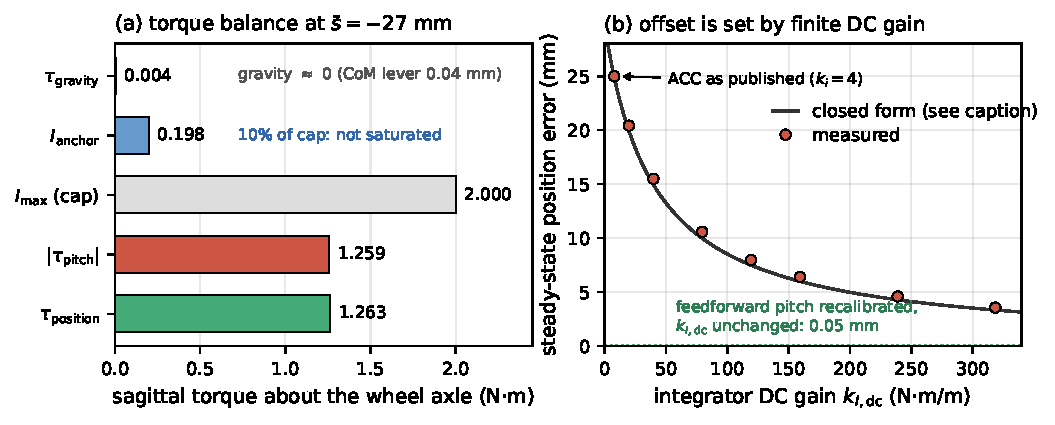
\includegraphics[width=\linewidth]{figures/parking_offset.pdf}
    \caption{Static torque balance of the sagittal parking offset.
    (a) Measured sagittal torques at the $\bar{s}{=}\SI{-27}{mm}$ parking point.
    The gravity moment about the wheel axle is \SI{0.0034}{Nm} and the anchor
    integral sits at \SI{10}{\percent} of its clamp, so the offset is neither
    gravity-driven nor a saturation artifact; the balance is between the
    pitch and position loops.
    (b) Steady-state position error against integrator DC gain
    $k_{I,\text{dc}}$ of Eq.~\eqref{eq:kidc}, swept over $k_i\in[4,160]$ at
    fixed leak. The curve is Eq.~\eqref{eq:parking} evaluated with the
    baseline $\tau_{\text{pitch}}$; using each run's own measured
    $\tau_{\text{pitch}}$ the closed form tracks all twelve gain and height
    points to within \SI{0.92}{\percent}. The dotted line is the same
    controller with the feedforward pitch reference recalibrated and
    $k_{I,\text{dc}}$ left unchanged.}
    \label{fig:parking}
\end{figure}

\subsection{Validation across a forty-fold gain sweep}

Sweeping $k_i$ from \num{4} to \num{160} at fixed leak moves $k_{I,\text{dc}}$
over $40{\times}$ and the offset follows Eq.~\eqref{eq:parking} throughout
(Fig.~\ref{fig:parking}b):

\begin{center}\footnotesize
\begin{tabular}{rrrrr}
\hline
$k_i$ & $k_{I,\text{dc}}$ & $e$ meas. & $e$ pred. & window jitter \\
 & (Nm/m) & (mm) & (mm) & (mm) \\
\hline
\textbf{4} & \textbf{7.96} & \textbf{-24.99} & \textbf{-24.87} & \textbf{0.298} \\
10 & 19.90 & -20.42 & -20.34 & 0.302 \\
20 & 39.80 & -15.49 & -15.54 & 0.147 \\
40 & 79.60 & -10.57 & -10.67 & 0.208 \\
60 & 119.40 & -7.96 & -8.01 & 0.168 \\
80 & 159.20 & -6.40 & -6.41 & 0.094 \\
120 & 238.80 & -4.59 & -4.58 & 0.114 \\
160 & 318.40 & -3.56 & -3.56 & 0.066 \\
\hline
\end{tabular}
\end{center}

Steadiness improves monotonically with $k_i$ over this range rather than
degrading, which is the opposite of the integral/steadiness trade-off measured
at $k_i{=}0$ in Table~\ref{tab:standing} and indicates that the $3{\times}$
steadiness cost reported there is paid at the first newton-metre of integral
authority, not progressively.

\subsection{The leak sets memory, not accuracy}

Because $k_{I,\text{dc}}$ depends on both $k_i$ and $\lambda$, reducing the
leak also raises DC gain---but it is the wrong knob. Cutting
$\lambda$ from \num{5e-3} to \num{5e-4} raises $k_{I,\text{dc}}$ to
\SI{79.96}{Nm/m} and does reduce the offset to \SI{-16.31}{mm}, but window
jitter degrades from \SI{0.298}{mm} to \SI{3.463}{mm}, a factor of \num{12},
and the measured error (\SI{-14.34}{mm}) does not reach its DC prediction
(\SI{-10.41}{mm}) because the forgetting time constant
$\tau{=}\Delta t/\lambda$ has grown to \SI{20}{s} and no longer settles inside
the measurement window. Since $\tau$ is independent of $k_i$, the two
parameters separate cleanly: $k_i$ sets DC gain, $\lambda$ sets the memory
horizon. They were conflated in the original tuning, where $\lambda$ was chosen
for a \SI{2}{s} forgetting time and $k_i$ was lowered from \num{8} to \num{4}
to reduce limit cycling---which, per the sweep above, cost accuracy without
buying steadiness.

\subsection{Two measured corrections and their cost}

The height dependence of the calibration error was checked on the five
posture-calibrated height variants, applying the correction measured at each
point:

\begin{center}\footnotesize
\begin{tabular}{rrrrr}
\hline
$h$ (m) & correction & $\bar{s}$ before & $\bar{s}$ after & reduction \\
 & (\SI{}{\degree}) & (mm) & (mm) & \\
\hline
0.394 & $-1.622$ & $-28.77$ & $-1.16$ & \SI{96.0}{\percent} \\
0.399 & $-1.974$ & $-34.53$ & $-1.20$ & \SI{96.5}{\percent} \\
\textbf{0.404} & $\mathbf{-1.461}$ & $\mathbf{-26.96}$ & $\mathbf{-2.02}$ & \textbf{\SI{92.5}{\percent}} \\
0.409 & $-0.943$ & $-19.29$ & $-2.83$ & \SI{85.3}{\percent} \\
0.414 & $-1.295$ & $-25.11$ & $-2.92$ & \SI{88.4}{\percent} \\
\hline
\end{tabular}
\end{center}

The controller's own position error falls to ${\leq}\SI{0.12}{mm}$ at every
height and the anchor integral to \SI{0.4}{\percent} of its clamp; what remains
is the \SIrange{1}{3}{mm} frame-convention gap. The required correction is not
a constant (it spans \SIrange{0.94}{1.97}{\degree} over \SI{2}{cm}), so this is
a per-height recalibration of the feedforward map rather than a single scalar.

Both corrections were then put through the full push protocol of
\S\ref{sec:push} ($N{=}10$ repetitions $\times$ 8 bearings, binary search over
\SIrange{10}{160}{N} at \SI{5}{N} tolerance; Welch's $t$ against the published
arm):

\begin{center}\footnotesize
\begin{tabular}{lrr}
\hline
Arm & $F_{\min}$ (N) & $F_{\text{med}}$ (N) \\
\hline
ACC as published ($k_i{=}4$) & 82.8(10) & 116.8(47) \\
$k_i{=}40$ & 81.8(18)\,\,$p{=}0.14$ & 116.8(70)\,\,$p{=}0.98$ \\
$k_i{=}160$ & 81.9(27)\,\,$p{=}0.32$ & 115.3(36)\,\,$p{=}0.43$ \\
Feedforward pitch recalibrated & 82.5(12)\,\,$p{=}0.55$ & 112.4(49)\,\,$p{=}0.05$ \\
\hline
\end{tabular}
\end{center}

The published arm reproduces the \SI{82.8}{N} weakest bearing of
\S\ref{sec:push} exactly, validating the harness. Raising $k_i$ by $40{\times}$
costs nothing measurable on either statistic and removes \SI{80}{\percent} of
the offset; the feedforward recalibration removes \SI{92.5}{\percent} and
leaves $F_{\min}$ unchanged, but shows a \SI{4.5}{N} (\SI{3.8}{\percent})
reduction in $F_{\text{med}}$ at $p{=}0.051$, which at this sample size we
report as unresolved rather than as null. Neither correction is promoted into
the shipped profile for this paper, because every table reported here was
measured on the published configuration and adopting a change would invalidate
that evidence base; they are reported as measured, reproducible routes to
closing the limitation.

\begin{thebibliography}{99}
\setlength{\itemsep}{0pt}
\setlength{\parsep}{0pt}
\setlength{\topsep}{0pt}

\bibitem{klemm2019ascento}
V.~Klemm \emph{et al.},
``Ascento: A Two-Wheeled Jumping Robot,''
in \emph{Proc. IEEE Int. Conf. Robotics and Automation (ICRA)}, 2019.

\bibitem{klemm2020lqrwbc}
V.~Klemm, A.~Morra, L.~Gulich, \emph{et al.},
``LQR-Assisted Whole-Body Control of a Wheeled Bipedal Robot with Kinematic Loops,''
\emph{IEEE Robotics and Automation Letters}, vol.~5, no.~2, pp. 3745--3752, 2020.

\bibitem{diablo2024}
D.~Liu \emph{et al.},
``DIABLO: A 6-DoF Wheeled Bipedal Robot Composed Entirely of Direct-Drive Joints,''
\emph{arXiv preprint arXiv:2407.21500}, 2024.

\bibitem{whleaper2024}
Y.~Zhu, S.~He, Z.~Qi, Z.~Yong, Y.~Qin, and J.~Chen,
``Whleaper: A 10-DOF Flexible Bipedal Wheeled Robot,''
in \emph{Proc. IEEE/RSJ Int. Conf. Intelligent Robots and Systems (IROS)}, pp. 11272--11277, 2024.

\bibitem{skater2024}
Y.~Wang, T.~Chen, X.~Rong, G.~Zhang, Y.~Li, and Y.~Xin,
``Design and Control of SKATER: A Wheeled-Bipedal Robot With High-Speed Turning Robustness and Terrain Adaptability,''
\emph{IEEE/ASME Trans. Mechatronics}, vol.~30, no.~2, pp. 1310--1321, 2025.

\bibitem{chamorro2024stairclimbing}
S.~Chamorro, V.~Klemm, M.~de~la~Iglesia~Valls, C.~Pal, and R.~Siegwart,
``Reinforcement Learning for Blind Stair Climbing with Legged and Wheeled-Legged Robots,''
in \emph{Proc. IEEE Int. Conf. Robotics and Automation (ICRA)}, 2024.

\bibitem{roscia2023flight}
F.~Roscia, A.~Cumerlotti, A.~Del~Prete, C.~Semini, and M.~Focchi,
``Orientation Control System: Enhancing Aerial Maneuvers for Quadruped Robots,''
\emph{Sensors}, vol.~23, no.~3, 1234, 2023.

\bibitem{englsberger2015dcm}
J.~Englsberger, C.~Ott, and A.~Albu-Sch\"{a}ffer,
``Three-Dimensional Bipedal Walking Control Based on Divergent Component of Motion,''
\emph{IEEE Trans. Robotics}, vol.~31, no.~2, pp. 355--368, 2015.

\bibitem{feng2023lqradrc}
X.~Feng, S.~Liu, Q.~Yuan, J.~Xiao, and D.~Zhao,
``Research on Wheel-Legged Robot Based on LQR and ADRC,''
\emph{Scientific Reports}, vol.~13, 15122, 2023.

\bibitem{ohnishi1993dob}
K.~Ohnishi, M.~Shibata, and T.~Murakami,
``Motion Control for Advanced Mechatronics,''
\emph{IEEE/ASME Trans. Mechatronics}, vol.~1, no.~1, pp. 56--67, 1996.

\bibitem{chen2000dob}
W.-H.~Chen, D.~J.~Ballance, P.~J.~Gawthrop, and J.~O'Reilly,
``A Nonlinear Disturbance Observer for Robotic Manipulators,''
\emph{IEEE Trans. Industrial Electronics}, vol.~47, no.~4, pp. 932--938, 2000.

\bibitem{han2009adrc}
J.~Han,
``From PID to Active Disturbance Rejection Control,''
\emph{IEEE Trans. Industrial Electronics}, vol.~56, no.~3, pp. 900--906, 2009.

\bibitem{bellicoso2016terrain}
C.~D.~Bellicoso, C.~Gehring, J.~Hwangbo, P.~Fankhauser, and M.~Hutter,
``Perception-Less Terrain Adaptation Through Whole Body Control and Hierarchical Optimization,''
in \emph{Proc. IEEE-RAS Int. Conf. Humanoid Robots (Humanoids)}, pp. 558--564, 2016.

\bibitem{bellicoso2018wbc}
C.~D.~Bellicoso, F.~Jenelten, C.~Gehring, and M.~Hutter,
``Dynamic Locomotion Through Online Nonlinear Motion Optimization for Quadrupedal Robots,''
\emph{IEEE Robotics and Automation Letters}, vol.~3, no.~3, pp. 2261--2268, 2018.

\bibitem{cascade_standard}
K.~J.~\AA{}str\"{o}m and T.~H\"{a}gglund,
\emph{PID Controllers: Theory, Design, and Tuning}, 2nd~ed.\ Instrument Society of America, 1995.

\bibitem{astrom2005advanced}
K.~J.~\AA{}str\"{o}m and T.~H\"{a}gglund,
\emph{Advanced PID Control}, ISA, 2006.

\bibitem{shinskey1996}
F.~G.~Shinskey,
\emph{Process Control Systems: Application, Design, and Tuning}, 4th~ed.\ McGraw-Hill, 1996.

\bibitem{gain_scheduling_survey}
W.~J.~Rugh and J.~S.~Shamma,
``Research on Gain Scheduling,''
\emph{Automatica}, vol.~36, no.~10, pp. 1401--1425, 2000.

\bibitem{boston_dynamics_handle2017}
Boston Dynamics,
``Introducing Handle,''
\emph{YouTube video}, Mar. 2017. [Online]. Available: \url{https://youtu.be/-7xvqQeoA8c}

\bibitem{swissmile2021}
M.~Bjelonic, P.~K.~Sankar, C.~D.~Bellicoso, and M.~Hutter,
``Proprioceptive Control for Hybrid Wheeled-Legged Locomotion: The Swiss-Mile Experience,''
in \emph{Proc. IEEE Int. Conf. Robotics and Automation (ICRA)}, pp. 6088--6095, 2021.

\bibitem{wada2019biteno}
T.~Wada, T.~Kinugasa, K.~Yoshida, and Y.~Sugahara,
``Development of a Wheeled Biped Robot ``BITeno'' Using Reaction Wheel Stabilization,''
\emph{J. Robotics and Mechatronics}, vol.~31, no.~5, pp. 729--738, 2019.

\bibitem{grimminger2020torque}
F.~Grimminger, A.~Meduri, M.~Khadiv, J.~Viereck, M.~W\"{u}thrich, L.~Wellhausen, \emph{et al.},
``An Open Torque-Controlled Modular Robot Architecture for Legged Locomotion Research,''
\emph{IEEE Robotics and Automation Letters}, vol.~5, no.~2, pp. 3650--3657, 2020.

\bibitem{herzog2016wbc}
A.~Herzog, N.~Rotella, S.~Mason, F.~Grimminger, S.~Schaal, and L.~Righetti,
``Momentum Control with Hierarchical Inverse Dynamics on a Torque-Controlled Humanoid,''
\emph{Autonomous Robots}, vol.~40, no.~3, pp. 473--491, 2016.

\bibitem{schulman2017ppo}
J.~Schulman, F.~Wolski, P.~Dhariwal, A.~Radford, and O.~Klimov,
``Proximal Policy Optimization Algorithms,''
\emph{arXiv preprint arXiv:1707.06347}, 2017.

\bibitem{hwangbo2019rl}
J.~Hwangbo, J.~Lee, A.~Dosovitskiy, D.~Bellicoso, V.~Tsounis, V.~Koltun, and M.~Hutter,
``Learning Agile and Dynamic Motor Skills for Legged Robots,''
\emph{Science Robotics}, vol.~4, no.~26, eaau5872, 2019.

\bibitem{pratt2006capturepoint}
J.~Pratt, J.~Carff, S.~Drakunov, and A.~Goswami,
``Capture Point: A Step Toward Humanoid Push Recovery,''
in \emph{Proc. IEEE-RAS Int. Conf. Humanoid Robots}, pp. 200--207, 2006.

\bibitem{legged_terrain_extero}
M.~Hutter \emph{et al.},
``ANYmal---Toward Legged Robots for Harsh Environments,''
\emph{Advanced Robotics}, vol.~31, no.~17, pp. 918--931, 2017.

\bibitem{blind_terrain_proprio}
G.~Bledt \emph{et al.},
``Contact Model Fusion for Event-Based Locomotion in Unstructured Terrains,''
in \emph{Proc. IEEE Int. Conf. Robotics and Automation (ICRA)}, pp. 4399--4406, 2018.

\bibitem{liu2024review}
X.~Liu, Y.~Sun, S.~Wen, K.~Cao, Q.~Qi, X.~Zhang, H.~Shen, G.~Chen, J.~Xu, and A.~Ji,
``Development of Wheel-Legged Biped Robots: A Review,''
\emph{Journal of Bionic Engineering}, vol.~21, no.~2, pp. 607--634, 2024.

\bibitem{mujoco}
E.~Todorov, T.~Erez, and Y.~Tassa,
``MuJoCo: A Physics Engine for Model-Based Control,''
in \emph{Proc. IEEE/RSJ Int. Conf. Intelligent Robots and Systems (IROS)}, pp. 5026--5033, 2012.

\bibitem{zamani2020coupled}
M.~Zamani, R.~Orr, and H.~Sadjadi,
``A Coupled 3D LQR for Two-Wheeled Balancing Robots,''
in \emph{Proc. IEEE Int. Conf. Robotics and Automation (ICRA)}, pp. 8761--8767, 2020.

\bibitem{cui2019dob}
R.~Cui, Y.~Li, and W.~Yan,
``Disturbance Observer Based Control for a Wheeled Bipedal Robot,''
\emph{IEEE Access}, vol.~7, pp. 112531--112540, 2019.

\bibitem{xin2022centroidal}
Y.~Xin, T.~Chen, and X.~Rong,
``Centroidal Dynamics for Coupled Pitch-Roll Control of Wheeled Bipedal Robots,''
\emph{IEEE Robotics and Automation Letters}, vol.~7, no.~4, pp. 10892--10899, 2022.

\bibitem{hyon2007gated}
S.-H.~Hyon and G.~Cheng,
``Gravity Compensation and Full-Body Balancing for Humanoid Robots,''
in \emph{Proc. IEEE-RAS Int. Conf. Humanoid Robots}, pp. 214--221, 2007.

\bibitem{liberzon2003switching}
D.~Liberzon,
\emph{Switching in Systems and Control},
Birkh\"{a}user, 2003.

\end{thebibliography}

\end{document}
